\documentclass[11pt, a4paper, oneside]{article}

\usepackage[portuguese]{babel}
\usepackage[utf8]{inputenc}
\usepackage{geometry}
\usepackage{booktabs}
\usepackage[figuresleft]{rotating}
\usepackage[pages=some,placement=centering]{background}

\geometry{
left   = 30mm,
right = 30mm,
top   = 30mm,
bottom=30mm,
}

\usepackage{color}   %May be necessary if you want to color links
\usepackage{hyperref}
\hypersetup{
    colorlinks=true, %set true if you want colored links
    linktoc=all,     %set to all if you want both sections and subsections linked
    linkcolor=blue,  %choose some color if you want links to stand out
}
\usepackage{graphicx}
\usepackage{amssymb, amsmath, amsthm}

\usepackage{fancyhdr}
\pagestyle{fancy}

\usepackage[pages=some,placement=centering]{background}

\usepackage{url}

\providecommand{\keywords}[1]{\textbf{\textit{keywords---}} #1}

\title{Simulação e Construção de um Equalizador de tensão Aplicado a Células Ultra-Capacitivas}
\author{Aluno : Fabiano Aparecido Marino \\NºUsp : 7143980 \\Orientador : Prof. Dr. Ricardo Quadros}

\begin{document}

 	\newpage
	\thispagestyle{empty}
	\clearpage
	\begin{sidewaysfigure}
		\centering
		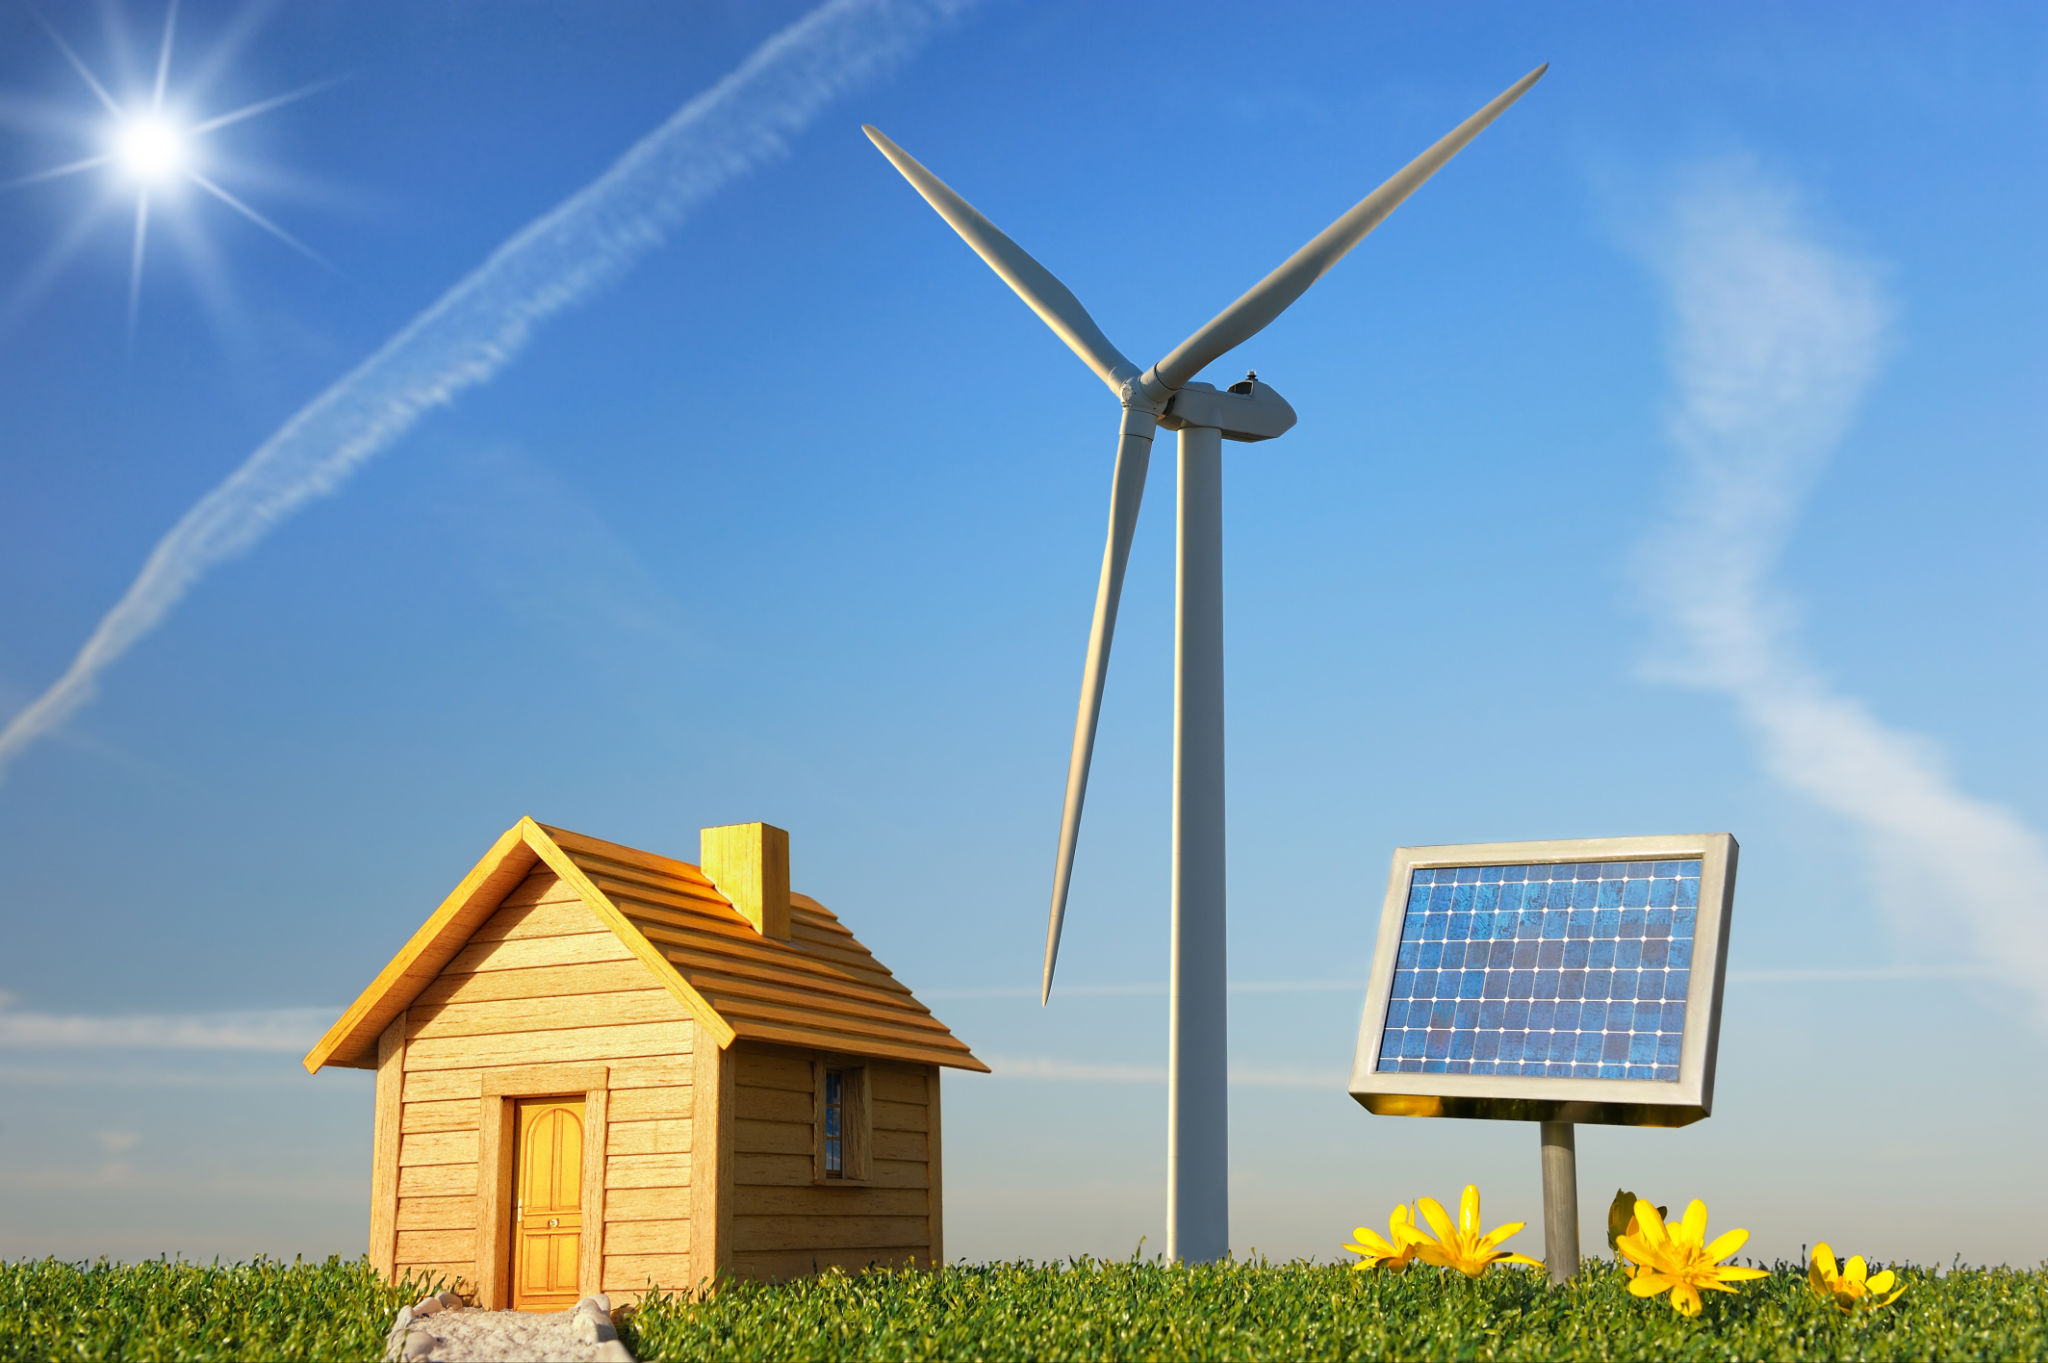
\includegraphics[width=1\linewidth]{capa_principal}
		\label{fig:adc_dac_ideal}
	
	\end{sidewaysfigure}
	\clearpage
	%\pagenumbering{gobble}
	\newpage

\maketitle

\begin{figure}[h!]
\centering
\includegraphics[width=1\linewidth]{capa.jpg}
\end{figure}

\newpage

\begin{abstract}
   A utilização de fontes alternativas de energia, tais como painéis fotovoltaicos,
células de combustível ou geradores eólicos, exigem o prévio armazenamento da
energia gerada e posterior envio para rede para garantir geração ininterrupta de
energia. No que se referem ao armazenamento de energia, os ultra-capacitores tem
fundamental importância quando se deseja manipular rápidos transientes de
energia.Para tanto, a sua utilização exige que a tensão em seus terminais seja
delicadamente controlada, desta forma, é necessário à construção de um sistema
equalizador de tensão. O principal objetivo deste projeto é a elaboração
de um sistema equalizador de tensão para ultra-capacitores que serão utilizados em
sistemas de geração distribuída de energia.
\end{abstract}

\keywords{ Eletrônica de pontência, Ultrapacitores, Fontes Alternativas de Energia, Equalizador de Tensão}


\begin{abstract}
The use of alternative energy sources such as photovoltaic panels,
fuel cells or wind generators, require the prior storage
energy generated and send to a network to ensure uninterrupted generation
energy. In referring to the energy storage capacitor has ultra-
crucial when you want to handle fast transients
energia.Para so, their use requires that the voltage at its terminals is
delicately controlled in this way, it is necessary to construct a system
voltage equalizer. The main objective of this project is to develop
a voltage equalizer system for ultra-capacitors that are used in
distributed power generation systems.
\end{abstract}

\keywords{ Power Electronic, Ultracapacitor, Alternative Source of Energy ,Voltage Equalizer}


\newpage

\tableofcontents
\listoffigures

\newpage

\section{\textit{Descrição das Capas}}

\subsubsection{\textit{Capa 1 : Abertura do Trabalho}}
\textit{Engenharia essa que busca maximizar os projetos por meio da aplicação tecnológica desenvolvida cuidadosamente.Porém, quem disse que os ponto de apoio final
do projeto não se baseiam em repostas, tais como, bom, belo, legal, lindo...\\
Isto vem trazer a imagem. Ambiente de aspectos naturais e vívidos com a simplicidade de uma casa pequena e aconchegante, utilizando das formas de geração energia 
presentes neste trabalho. O passivo do campo, com a maturidade da tecnologia aplicada, mais a fundo, a simplicidade embaraçada com o avanço tecnológico, permitindo
a coexistência do ser humano em compassividade com a natureza.}

\subsubsection{\textit{Capa 2 : Conjunto de Geradores Eólicos}}
\textit{Trata-se de uma subestação de geração de energia eólica, havendo a possibilidade de se verificar um possível local de aplicação da tecnologia, sendo, na presente imagem,
um lugar fugidio, longiquo, aonde , em países de avançado desenvolvimento, há a aplicação de tecnologia de ponta visando o suprimento de energia local ou em rede distribuida interligada.} 

\subsubsection{\textit{Capa 3 : Simulação da Colisão Hélice com Fluido}}
\textit{O principio de funcionamento das hélices eólicas geradoras de energia é o fato de que o ar, como fluido que é, uma vez entrando em colisão com a hélice
o faz girar, havendo utilização dos movimentos da hélice para geração de energia elétrica. Simulações que visem obter o comportamento do fluido em torno da hélice
é de grande importância, pois assim se dá o projeto de novas hélices que melhoram o rendimento do sistema.}

\subsubsection{\textit{Capa 4 : Roteamento de Placas em Várias Camadas}}
\textit{O roteamento de placas eletronicas se dá de forma a explorar o caminho da trilha tanto na horizontal como na vertical da placa, considerando um olhar sobre o plano da placa. 
A figura faz uma descompactação de uma placa roteada mostrando que há trilhas nas camadas que a compõem assim como toda a superfície.}

\newpage

\section{Fontes Alternativas de Energia}
Havendo a necessidade de se realizar trabalho, o homem buscou por meio
da engenharia diferentes formas de se obte-lá, aonde houve a tentativa de
retirá-la do movimento das águas, do carvão e, após uma grande evolução
tecnológica, viu-se que a conversão de uma forma de energia na outra e posterior e
armazenamento em bancos de baterias especializado nas formas de energia em
questão, é uma útil e eficiente forma de se lidar com as necessidades energéticas
de um grupo. Hoje em dia, uma grande parcela da energia total gerada é na forma
de eletricidade e é oriunda de usinas hidrelétricas e termoelétricas, sendo uma das
mais importantes fontes de energia alternatia. Como pontos fortes deste tipo de fonte de energia
pode-se citar fácil transporte por meio de sistemas de transmissão, além de fácil
armazenamento e bom domínio da tecnologia empregada, considerando o Brasil como aplicante da tecnologia citada.\\
Após um tempo de uso tais fontes passaram a expressar seus pontos
negativos que hoje se fazem bastante alarmantes: em primeiro lugar é possível
mencionar o aquecimento global que se relaciona diretamente com as fontes
citadas anteriormente, afinal a combustão do carvão, usado em termoelétricas, e do
petróleo, liberam gás carbônico que é o principal agente do efeito estufa. Outro
ponto a ser citado, e não de menor repercussão, são os alagamentos causados pelas
hidrelétricas em grandes áreas próximas a rios, devastando a mata da região e
sendo danoso ao micro-clima local.\cite{meio_ambiente}\\
Levando em consideração tais fatores, um importante objetivo da sociedade
moderna é buscar novas fontes de energia elétrica, que minimizem os efeitos
colaterais sobre o meio ambiente, visando reverter à situação de desequilíbrio
ambientais que o uso de combustíveis fósseis trouxe ao planeta.
Dentro desse contexto existem várias outras fontes de energia, como a
nuclear, por exemplo, que, dentre as formas alternativas, é a mais explorada.
Outros exemplos são as fontes que utilizam da energia solar irradiada sobre a
superfície terrestre, conhecida como fonte solar. Uma forma também alternativa é
utilização da energia presente no vento, chamada de usinas eólicas. Tais fontes já
estão em uso, apesar de ainda serem inespressivas quando comparada com a
quantia gerada por fontes térmicas e hidrelétricas. Abaixo encontram-se algumas
imagens de sistemas de geração de energia alternativos ao hidrelétrico.


\begin{figure}[h!]
  \centering
  \begin{minipage}[b]{0.45\textwidth}
    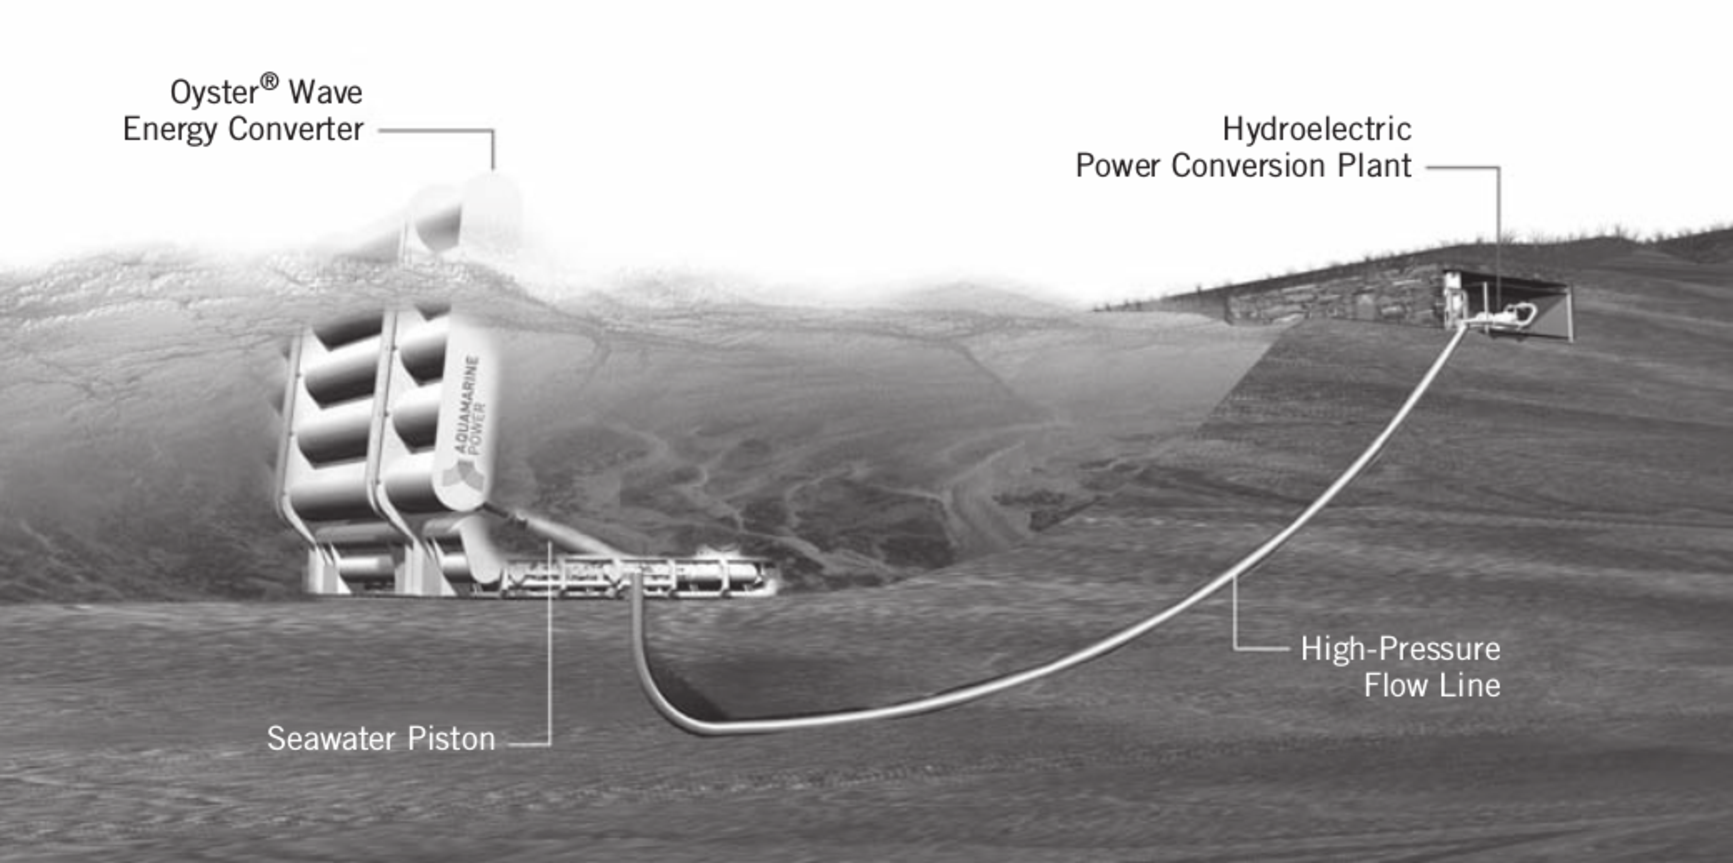
\includegraphics[width=\textwidth]{Alternative_energy2}
    \caption{Fonte de Alternativa via Movimento da água no Fundo do Mar \cite{mecanica_dos_fluidos}}
  \end{minipage}
  \hfill
  \begin{minipage}[b]{0.45\textwidth}
    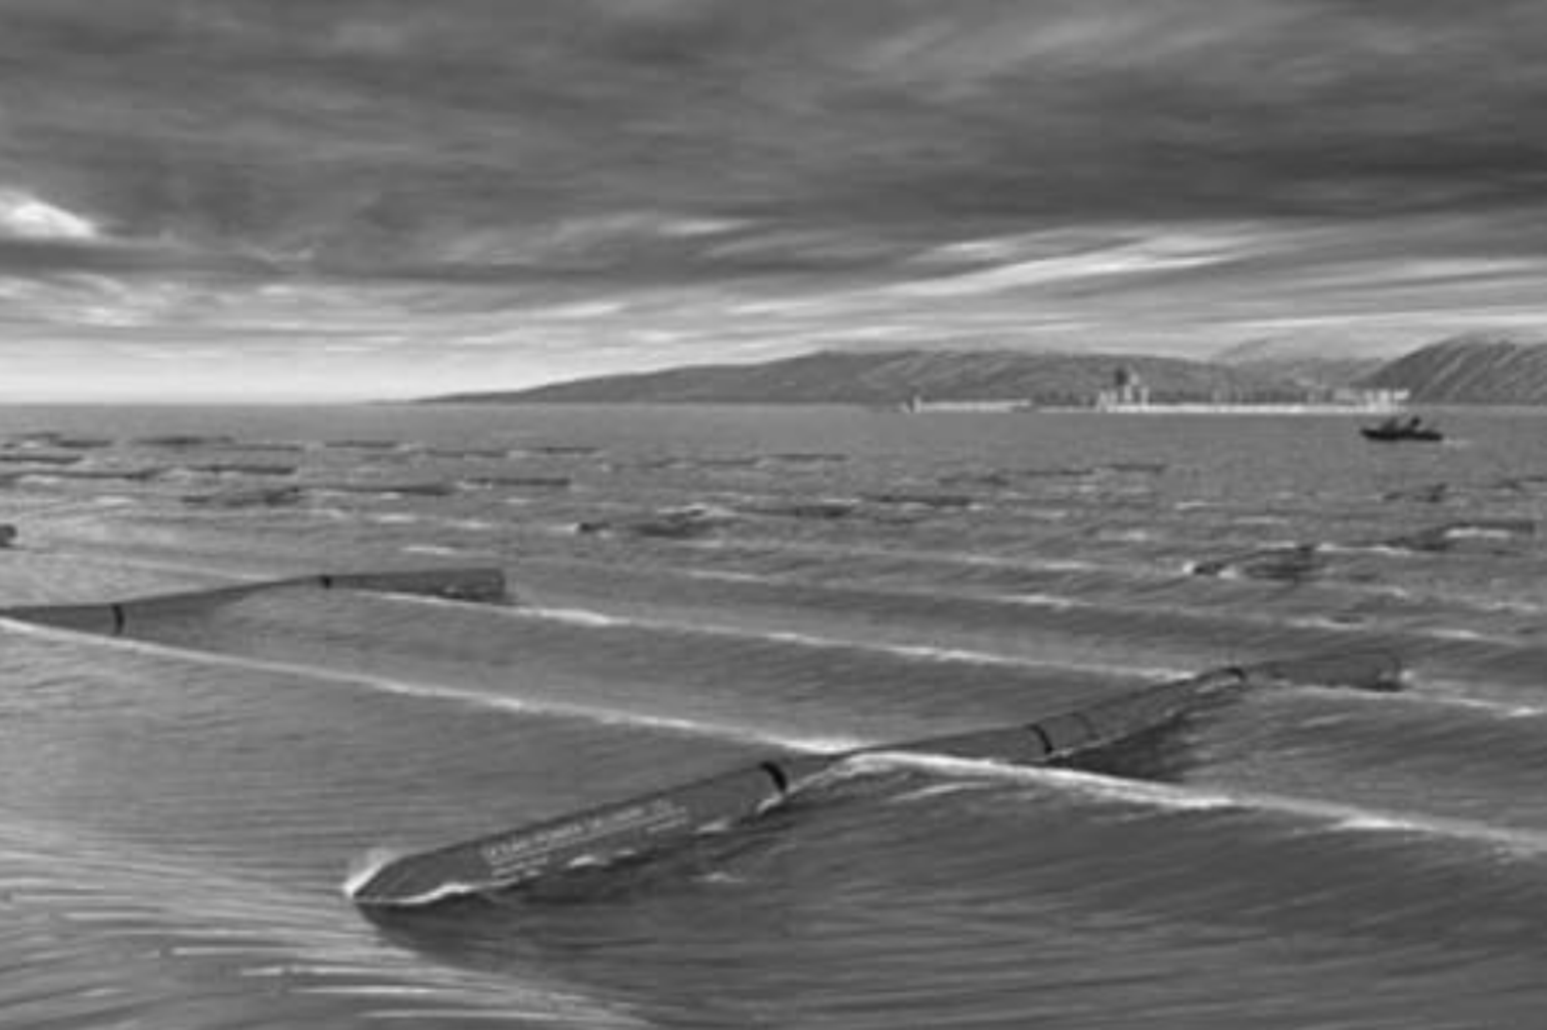
\includegraphics[width=\textwidth]{Alternative_energy1}
    \caption{Fonte Alternativa via Movimento da Água do Mar na superfície \cite{mecanica_dos_fluidos}}
  \end{minipage}
\end{figure}

Ambas as imagens expressam estruturas que retiram energia da água,
porém não do fluxo que passa por uma turbina, assim como acontece nos modelos de
geração hidrelétrica comum, o que exige armazenamento de água em grandes
represas de armazenamento. A estrutura apresentada retira energia do balanço da
água, seja esse balanço no fundo do mar ou na superfície, assim como mostram as
imagens.Abaixo encontra-se uma imagem de uma estação de geração solar de
energia, construída por meio de espelhos que direcionam a luz solar a um único
ponto, que por sua vez aquece um container, aonde ocorre o aquecimento da água, que uma vez aquecida, quando posta pressão ambiente, sai em alta pressão por um
orificio que o direciona para uma turbina girando-a. A partir deste ponto o modo de geração da energia é semelhante ao hidrelétrico.

\begin{figure}[h!]
\centering
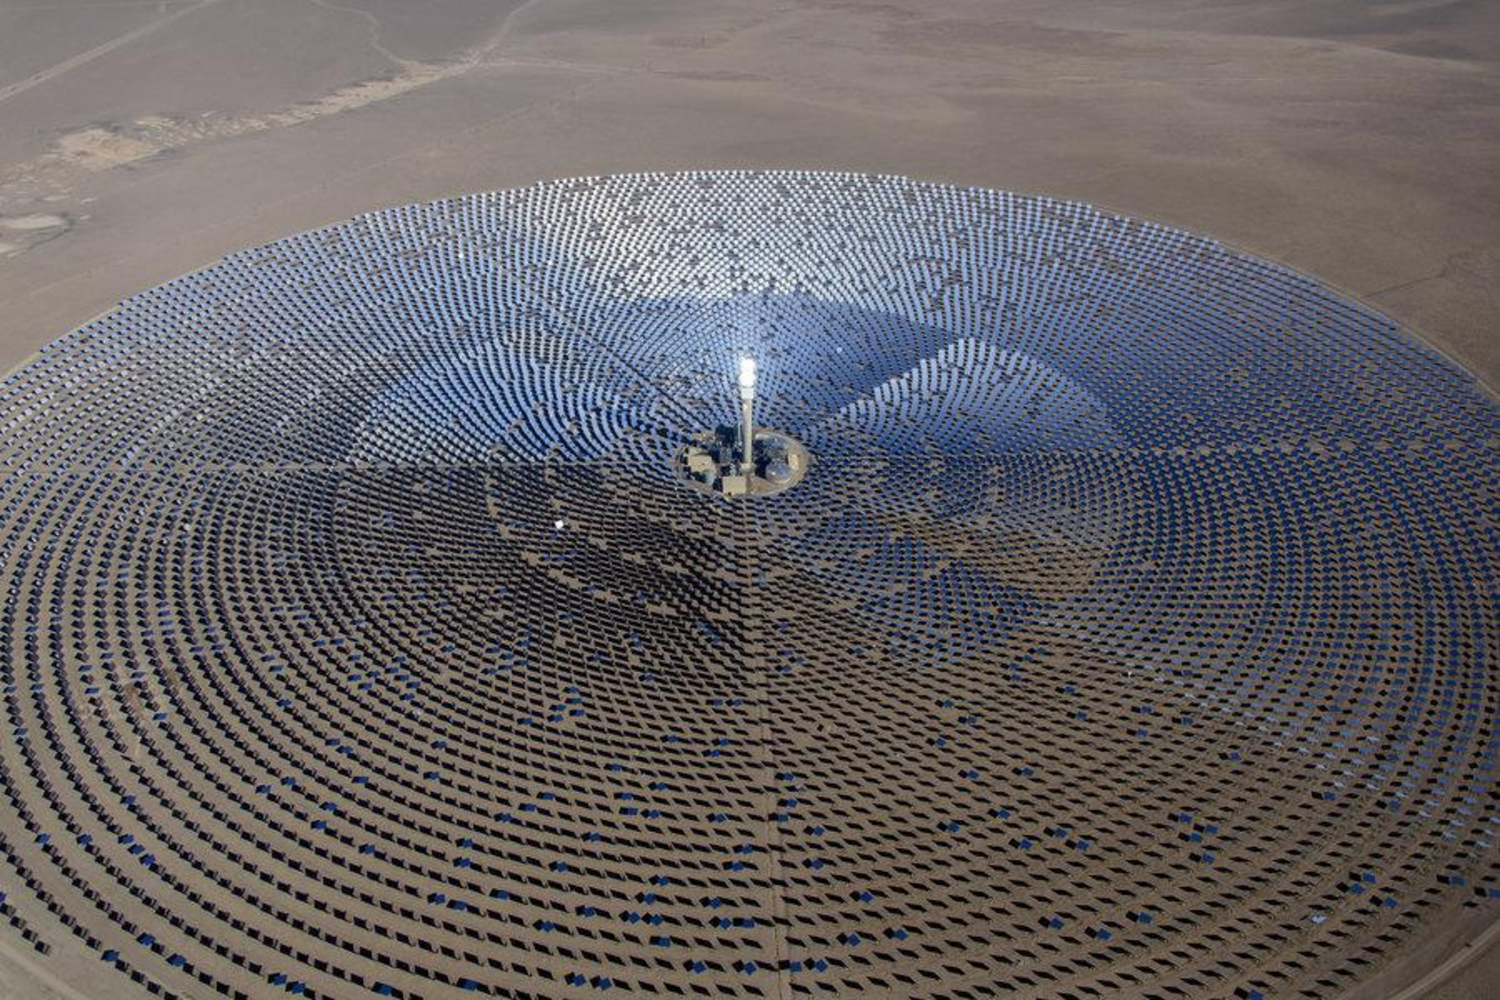
\includegraphics[width=1\linewidth]{fonte_solar}
\caption{Estação de Energia Solar \cite{fonte_solar}}
\end{figure}

A energia solar é bastante expressiva do ponto de vista do volume de
irradiação sobre a superfície do planeta. Anualmente, tal energia é maior do que a
soma das outras energias, contando ainda com baixo impacto ambiental, sendo
este um aspecto bastante favorável a sua utilização. Apesar disso, devido às perdas
e eficiência dos sistemas fotovoltaicos que são utilizados para captar irradiação e
transformá-la em energia elétrica, ainda não é possível ter o máximo
aproveitamento da energia da irradiação solar. A Figura (\ref{energias_planeta}) mostra a comparação
entre o potencial energético da irradiação solar anual da terra e o equivalente do
potencial energético comparando com as demais fontes de energia utilizadas.\\
Uma grande vantagem dos sistemas fotovoltaicos é o fato de que as
instalações de suas estações geradoras podem ser feitas em pequenas unidades, de
forma distribuída e próxima das cargas, contribuindo para a flexibilidade do seu
posicionamento e diminuindo a necessidade de sistemas de transmissão.

\begin{figure}[h!]
\centering
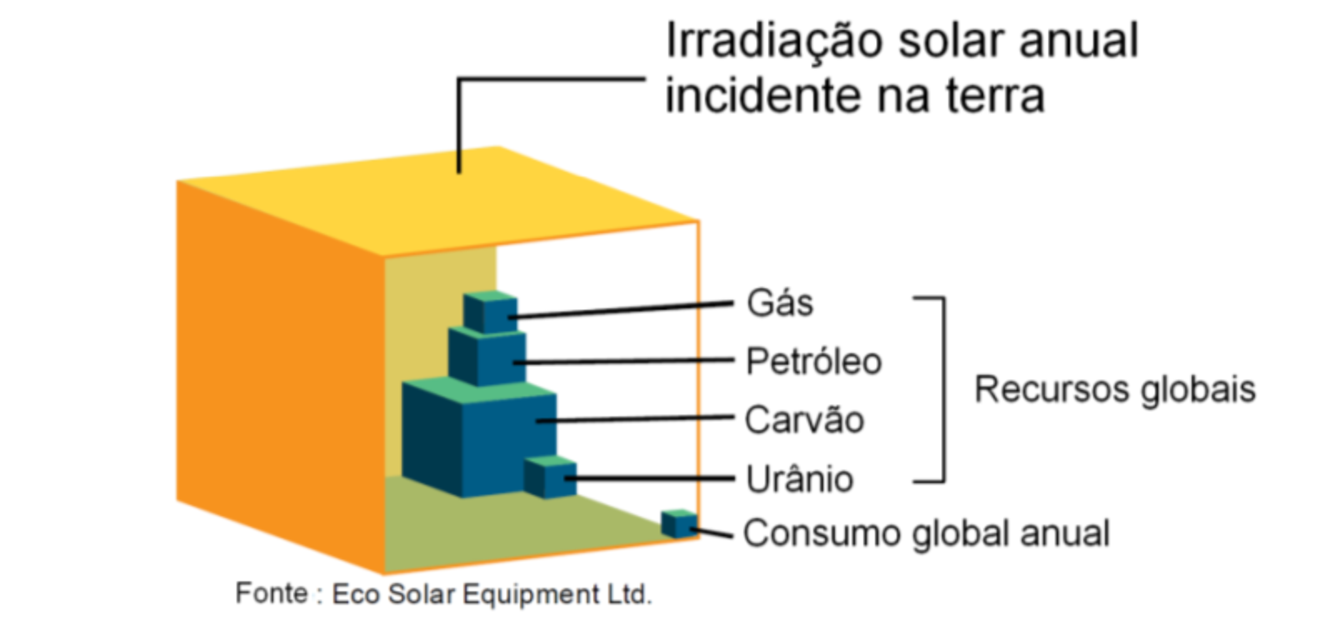
\includegraphics[width=.6\linewidth]{irradiacao_cada_energia}
\label{energias_planeta}
\caption{Quantidade de energia em proporção cosiderando cada fonte \cite{mestrado_renan}}
\end{figure}

Assim como as estações de geração solar podem ser construídas em
pequenas unidades, as fontes de geração eólica também fazem uso de tal
propriedade, tornando-as bastante versáteis quanto ao seu posicionamento,
limitando-se ao fato de que é fundamental a instalação em regiões com ventos
constantes para que haja o máximo aproveitamento desses sistemas.\\
Sistemas armazenadores de energia são necessários para essas fontes
devido à inconstância da geração, podendo inclusive ser nula em determinado
momento do dia, como em sistemas fotovoltaicos durante a noite (PV). Desta
forma, é necessário um estoque de energia para manter o fornecimento constante
quando houver ausência ou insuficiência da irradiação ou vento.\\
Sistemas de armazenamento baseado em baterias é uma solução viável para
acumulo de energia de sistemas solares ou eólicos, uma vez que elas são utilizadas para
grandes armazenamentos de energia e, posteriormente, utilizadas para fornecer
essa energia de forma contínua para a rede ou carga. Entretanto, as baterias não
são capazes de suprirem transitórios de energia, em que há a necessidade de
fornecimento de potência em curtos intervalos de tempo, logo, os ultra-capacitores
são essenciais para atuarem nessas situações, pois sua capacidade de rápida
descarga pode suprir a necessidade de transientes de potência para sistemas
conectados com a rede.\\
Na Figura (\ref{fig:estrutura_do_doutorado} tem-se um esquema da estruturação e integração das fontes
alternativas,sendo este o objetivo de montagem do trabalho de doutorado aque o
presente projeto de IC se direciona, na qual é mostrado um PV, banco de baterias e
ultra-capacitores conectados a um barramento cc através de conversores cc-cc e
um aerogerador conectado no mesmo barramento, através de um conversor ca-cc.\\
Na sequência, o barramento cc é ligado à rede através da interface de um
conversor cc-ca.Os equalizadores de tensão encontram-se conectados aos
terminais dos ultra-capacitores.

\begin{figure}[h!]
\label{fig:estrutura_do_doutorado}
\centering
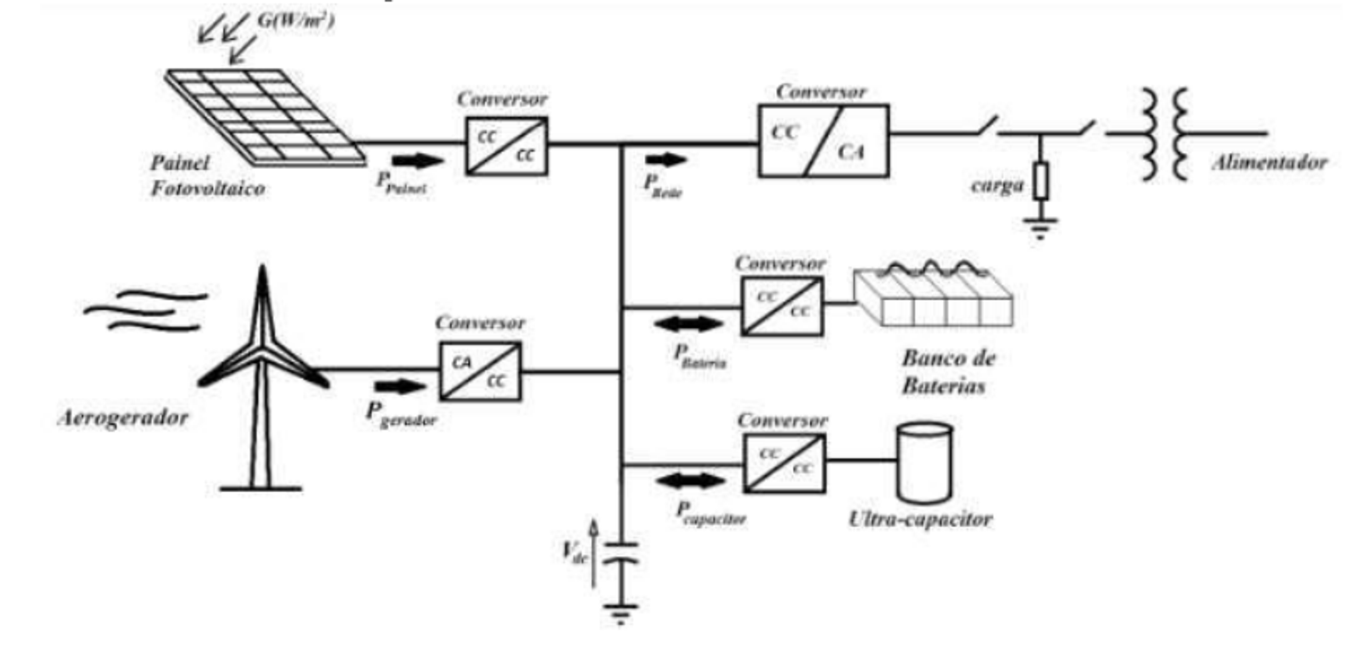
\includegraphics[width=1\linewidth]{Estrutura_de_geracao_eolica_solar}
\caption{Estrutura de geração eólica e solar com armazenamento em baterias e ultracapacitores \cite{mestrado_renan}}
\end{figure}

\newpage 


 	\newpage
	\thispagestyle{empty}
	\clearpage
	\begin{sidewaysfigure}
		\centering
		\includegraphics[width=1\linewidth]{capa1}
		\label{fig:adc_dac_ideal}
		\caption{Conjunto de Geradores Eólicos \textit{Descrição da Imagem em : Descrições de Capas}}
	\end{sidewaysfigure}
	\clearpage
	%\pagenumbering{gobble}
	\newpage
	
\section{Equalizadores de Tensão}
Muitos dos sistemas de geração de energia desenvolvidos possuem como
base uma fonte natural de força motriz, como exemplo pode-se citar as fontes
eólica e solar, além da hidráulica, oque os coloca dependentes dos fatoresclimáticos da região quanto à geração ou não de energia. Desse modo, a fim de
garantir o fornecimento em momentos de geração nula, como é o caso da geração
solar a noite, se faz necessário que a mesma seja armazenada para que
posteriormente ocorra seu consumo, conforme as necessidades solicitadas pela
rede.\\
Tendo esta questão em vista, se faz necessário o uso de elementos
armazenadores de energia, aonde tem-se como opções capacitores de grande
porte, mais conhecidos como ultra-capacitores e baterias. Os bancos de
armazenamento formados por baterias e ultra-capacitores constituem uma
estrutura bastante eficiente, haja vista que as baterias possuem alta capacidade de
armazenamento enquanto os ultra-capacitores não armazenam grandes quantias,
porém fornecem energia em alta potência, sendo muito eficientes em momentos de
pico de consumo. Aos sistemas de armazenamento formados por mais de um tipo
de elemento armazenador diz-se ser um sistema hibrido de armazenamento.\\
O banco armazenador é uma parte muito importante do projeto, pois o mau
funcionamento do mesmo compromete toda a estrutura, afinal é dele que sai a
energia para se realizar o trabalho a que o projeto foi direcionado. Para garantir o
seu ótimo funcionamento busca-se monitorar as grandezas que afetam seu
desempenho, como sua temperatura, processo de carga e descarga, estado de carga
e saúde dos elementos, tempo restante de vida e, além de outros, o balanceamento
da tensão ao longo das células de conexão entre os elementos armazenadores,
sendo este ultimo fator o mais relevante.\\
Por balanceamento de tensão, ou equalização de tensão, termo bastante
utilizado, entende-se como sendo o processo de atuar no sistema de modo a fazer
com que diferença de tensão nas células de armazenamento fique em torno de
valores próximos uma das outras, e, além disso, evitando que a célula com menor
tensão seja sobrecarregada no processo de carregamento.Muitos são os
sistemas desenvolvidos para realizar tal tarefa.Uma breve revisão das topologias
de equalização é feita neste trabalho, bem como a realização de simulações
utilizando o software Proteus.\\
Abaixo encontra-se um diagrama esquemático das diferentes maneiras de
se equalizar a tensão nos terminais das células de armazenamento, expressando o
grande número de sistemas desenvolvidos.Em primeira instância os
métodos de equalização dividem-se em passivos e ativos, o que classifica o
processo segundo o consumo ou não de energia ao equalizar a tensão nas células.
Dentro de cada um desses aspectos há outras subdivisões que versam quanto ao
elemento utilizado, que no caso ativo são resistores, e no passivo podem ser
capacitores, indutores ou conversores de energia. Para cada uma das
possibilidades de elemento utilizado há ainda divisões que referem-se ao processo
ser chaveado ou não e a características do elemento utilizado, como enrolamentos
da bobina indutora e o método de conversão dos conversores.

\begin{figure}[h!]
\label{fig:estrutura_do_doutorado}
\centering
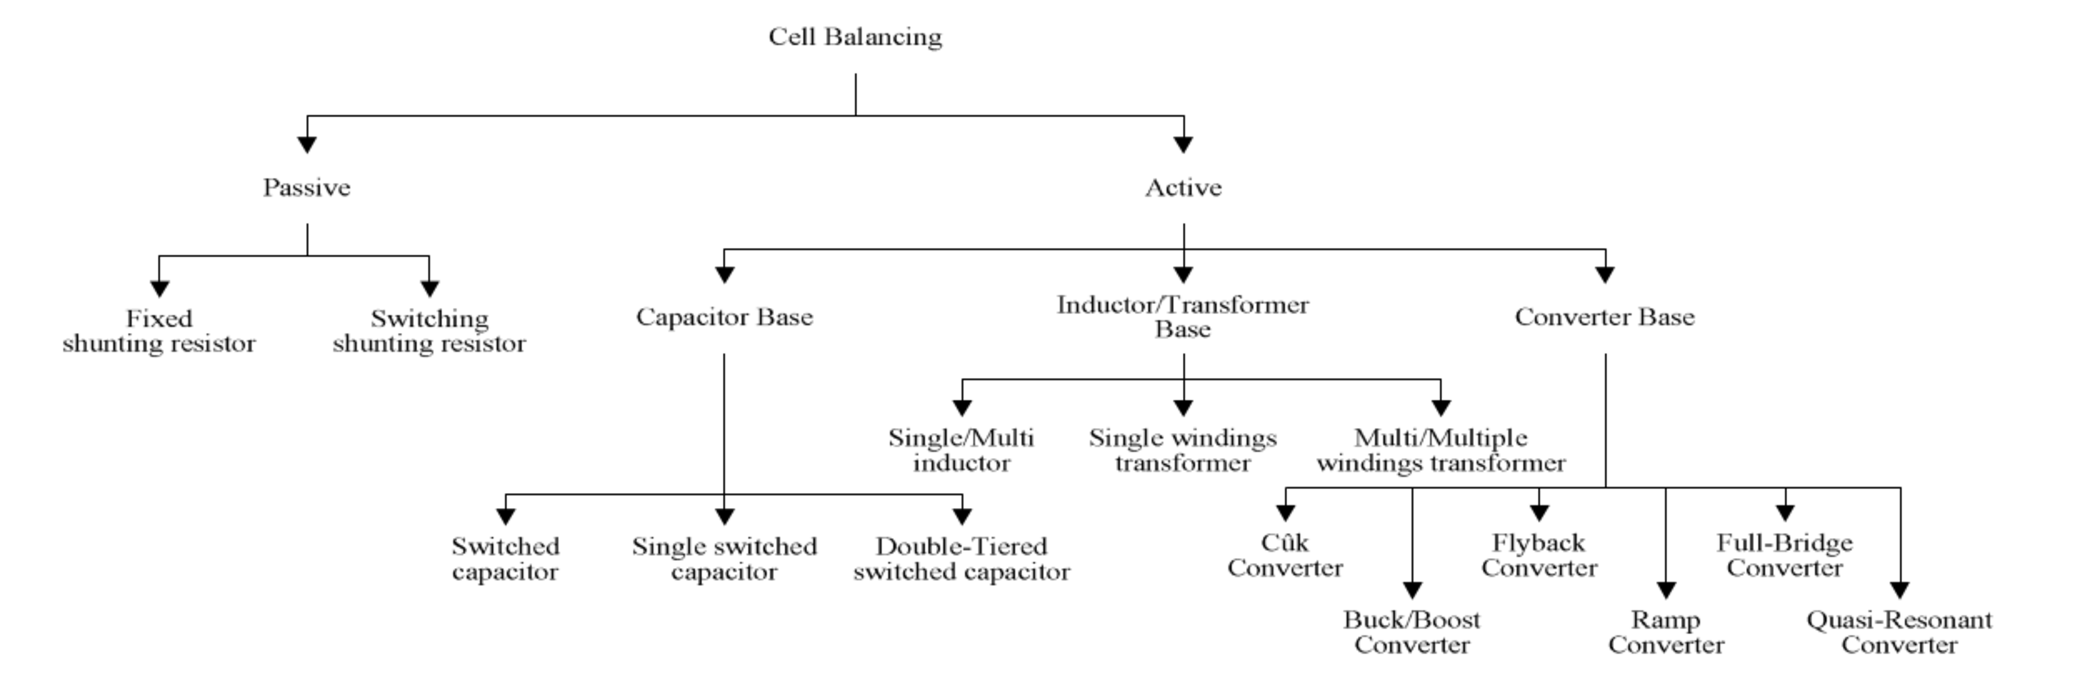
\includegraphics[width=1\linewidth]{topologia_de_equalizacao}
\caption{Topologias de Equalização \cite{energy_figure}}
\end{figure}

\subsection{Método Passivo}
Os métodos passivos caracterizam-se por permitirem o fluxo de energia das
células mais carregadas para as menos, sendo que esta passa por um componente
passivo pelo qual uma parte do excesso de energia armazenado em uma das
células é dissipado, de forma a levar tensão na referida célula ao seu valor
equalizado. Devido ao fato de que uma parte da energia armazenada é consumida
durante o processo de equalização este método não é eficiente, além de outros
entraves relacionados ao tempo de equalização.O resistor utilizado pode ser tanto
chaveado como fixo, dependendo da topologia utilizada.

\subsection{Método Ativo}
Estes métodos fazem o processo de equalização, ou seja, retiram energia das
células mais carregadas direcionando-a para as menos, sem que uma parte da
energia armazenada seja consumida. Dentre os elementos utilizados para realizar
a equalização encontram-se capacitores e indutores bem como conversores, sendo
que tais podem ser chaveados ou não.

\subsection{Fixed Shunting Resistor}
Consiste no mais simples dos métodos de equalização existente, pois é
constituído somente de um resistor por onde o excesso de energia presente nas
células mais carregadas é direcionado para as menos carregadas.O fluxo de energia
ocorre naturalmente, pois células mais carregadaspossuem a tensão em seus
terminais mais elevada e, lembrando que a corrente flui do maior para o menor
potencial, o fluxo ocorre naturalmente.Conforme a célula menos carregada recebe
energia a tensão em seus terminais aumenta gradualmente, até que seja igual a da
célula que estava com excesso de energia, terminando assim o processo de
equalização.\\
Uma das possibilidades deste método é utilizando um resistor fixo, que,
como foi descrito logo acima, é por onde a energia será transferida da célula maiscarregada para a menos carregada.Longo tempo de equalização além da
necessidade de um controle térmico, devido a constante dissipação de energia, são
características desta topologia que fazem dela um método pouco eficiente. A
figura (\ref{fig:estrutura_equalizador_shunting}) presente abaixo expressa a topologia deste circuito equalizador.

\newpage

\begin{figure}[h!]

\centering
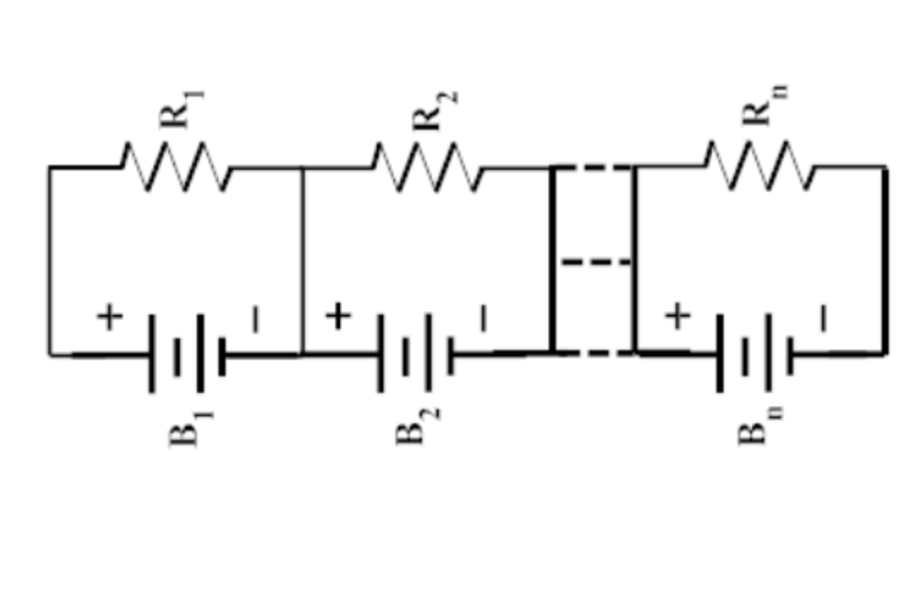
\includegraphics[width=0.5\linewidth]{equalizador_ativo}
\caption{Topologia de Equalização Shunting \cite{energy_figure}}
\label{fig:estrutura_equalizador_shunting}
\end{figure}

A outra possibilidade dentre os equalizadores shunting difere da
anteriormente apresentada apenas pela presença de uma chave na célula de
armazenamento, fazendo com que o fluxo de energia da célula mais carregada para
a menos não ocorra de maneira continua.Há, dentro deste tipo de topologia, dois
modos de se efetuar o chaveamento: o primeiro é monitorando todas as chaves de
um único modo, fazendo com que o processo de descarregamento não seja
contínuo, o outro utiliza um sistema inteligente de controle que verifica o
desbalanço de tensão para posteriormente chavear o sistema, sendo que a chave a
ser ativada é escolhida de modo que o processo seja o mais eficiente possível.A
figura (\ref{fig:estrutura_equalizador_shunting_controlado}) presente abaixo expressa esta topologia.

\begin{figure}[h!]
\centering
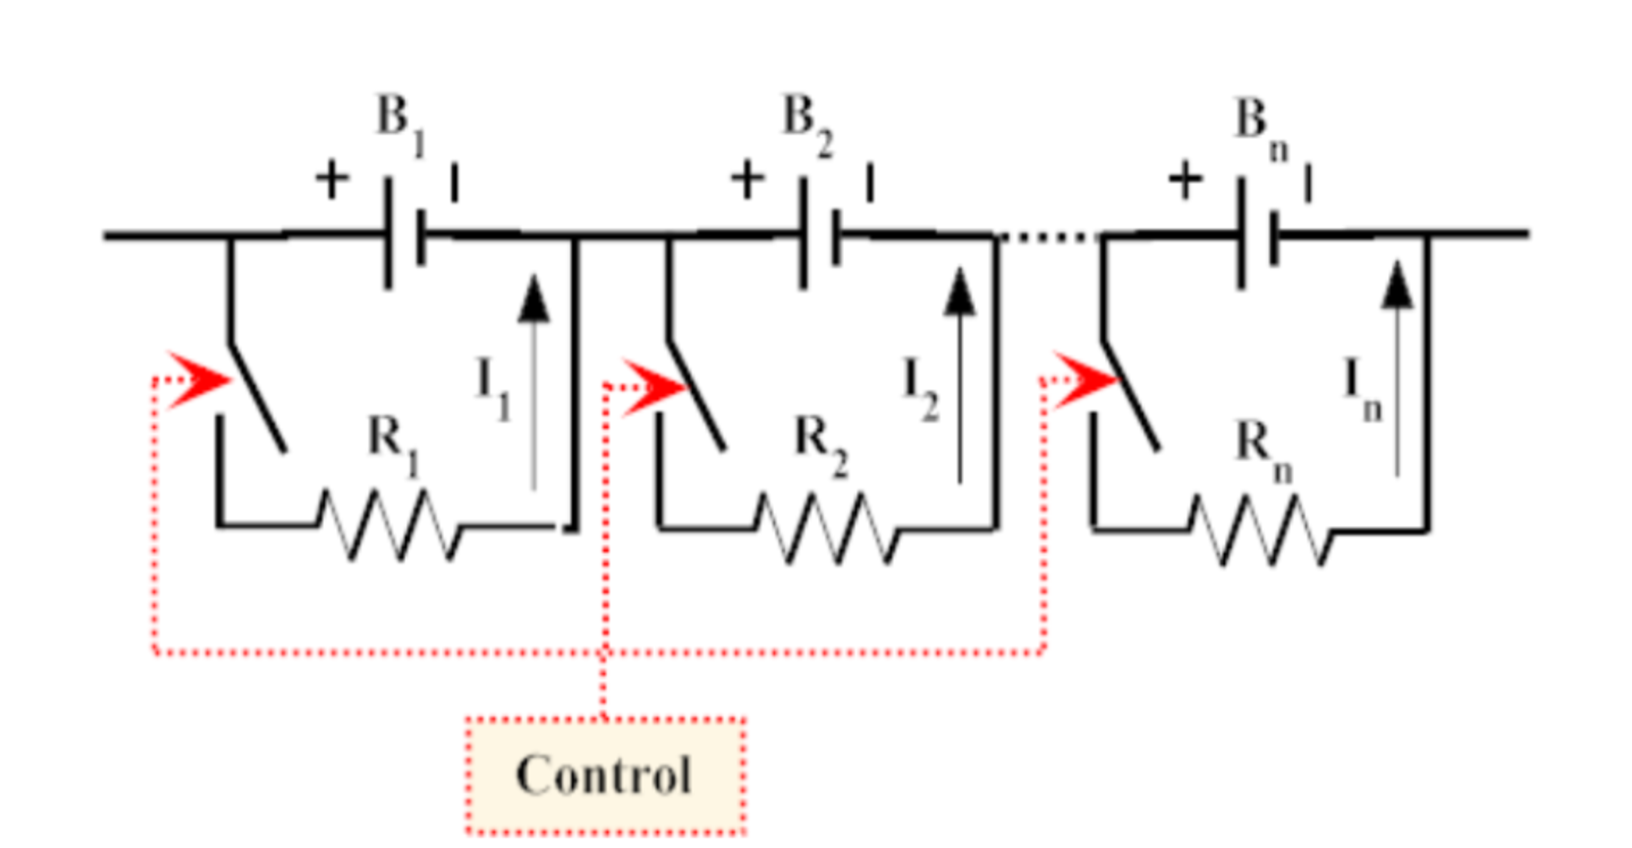
\includegraphics[width=0.6\linewidth]{ativo_com_controle}
\caption{Topologias de Equalização Shuntinhg Controlada \cite{energy_figure}}
\label{fig:estrutura_equalizador_shunting_controlado}
\end{figure}

Apesar de apresentar os mesmos entraves do método de equalização com
resistor fixo, esta topologia possui um tempo de equalização relativamente menor,
sendo uma característica positiva desta topologia.

\section{Métodos Passivos}

\subsection{Métodos Pelos Capacitores de Shunting}
Devido ao elemento utilizado para permitir o transporte de energia das
células mais carregadas para as menos deixar de ser um resistor, os sistemas de
equalização deixam de consumir uma parte da energia armazenada durante o
processo, passando a serem classificados como métodos passivos de
equalização.Um possível componente a se utilizar,ao invés de resistores, são os
capacitores, bastando que estes sejam conectados em paralelo com as células de
armazenamento.Tal topologia pode ser classificada em três categorias: capacitor
chaveado, capacitor chaveado único e capacitor duplo conectado.

\subsection{Capacitor Chaveado}
O método de equalização com capacitor chaveado requer n-1 capacitores e
2n chaves para balancear n células. O controle utilizado possui somente 2 estados ,
sem a necessidade de um controle inteligente. Pode atuar tanto no ciclo de carga
como de descarga, sendo uma desvantagem desta topologia seu longo tempo de
equalização. A figura (\ref{fig:estrutura_equalizador_passivo_ apacitor}), presente abaixo, ilustra esta topologia.

\begin{figure}[h!]
\centering
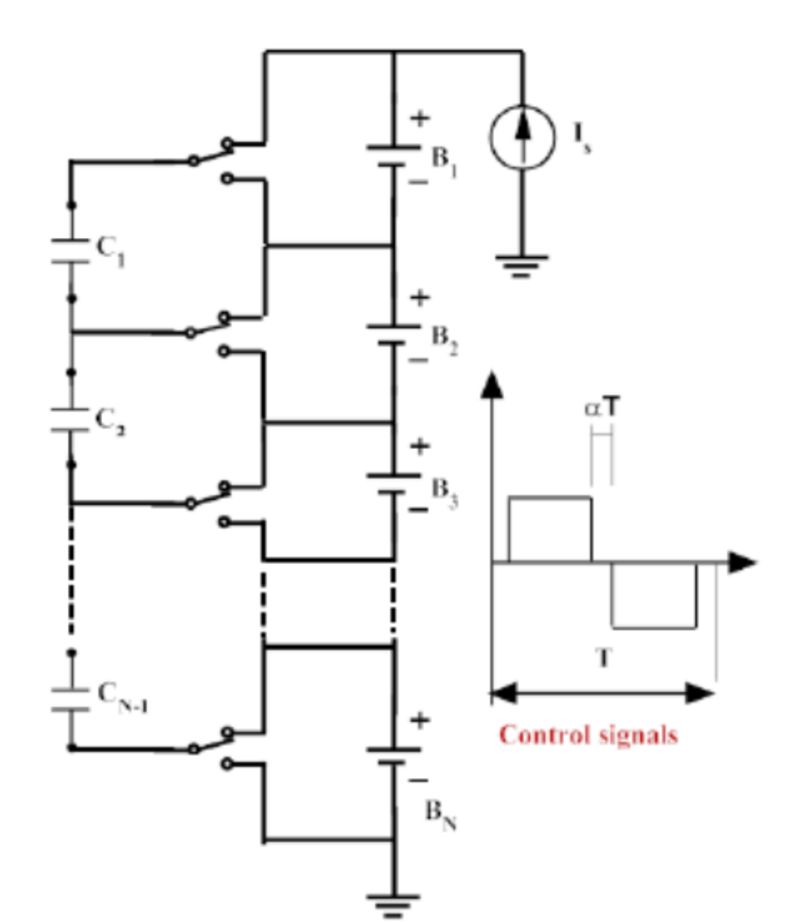
\includegraphics[width=0.6\linewidth]{topologia_equalizacao_capacitor_chaveado}
\caption{Topologias de Equalização com Capacitor Chaveado \cite{energy_figure}}
\label{fig:estrutura_equalizador_passivo_ apacitor}
\end{figure}

\subsection{Capacitor Único Chaveado}
Esta topologia pode ser considerada como uma derivação da topologia
capacitor chaveado, porém utiliza um único capacitor, como mostrado na Figura 5,
presente abaixo. Necessita n+5 chaves para balancear n células. A estratégia de
controle utilizada consiste na detecção da maior e menor diferença de potencial e
chaveia as correspondentes chaves de modo a permitir o fluxo de energia dentreestas células. 
Outras estratégias de controle podem ser utilizadas de modo a
diminuir o tempo de equalização.

\begin{figure}[h!]
\centering
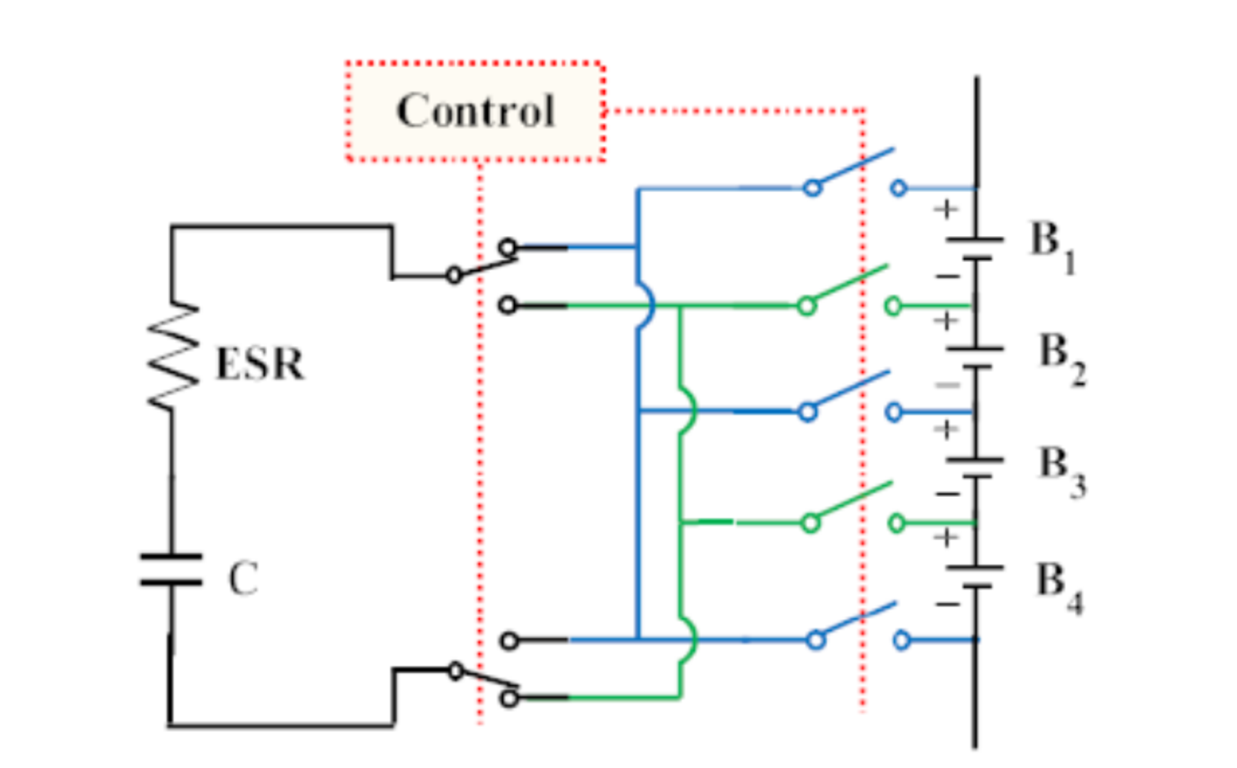
\includegraphics[width=0.6\linewidth]{capacitor_unico_chaveado}
\caption{Topologias de Equalização com Capacitor Chaveado \cite{energy_figure}}
\label{fig:estrutura_equalizador_passivo_ apacitor}
\end{figure}

\subsection{Capacitor Duplo Chaveado}
Também é uma derivação da topologia capacitor chaveado, sendo a
diferença relacionada ao uso da combinação de capacitores assim como ilustrado
na Figura 6, presente abaixo. Necessita de n capacitores e 2n chaves para
balancear n células.A vantagem desta topologia é que o segundo resistor presente
na malha reduz o tempo de equalização para um quarto do tempo necessário
relativamentea topologia capacitor chaveado. Uma outra propriedade é que este
atua tanto no ciclo de carga como descarga.	

\begin{figure}[h!]
\centering
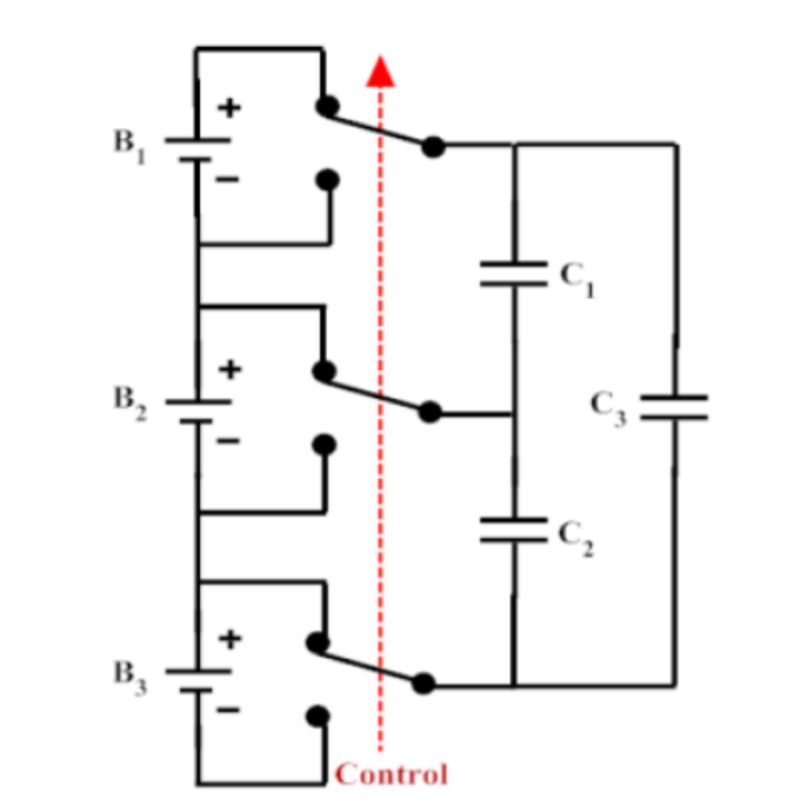
\includegraphics[width=0.6\linewidth]{capacitor_chaveado_duplo}
\caption{Topologias de Equalização com Capacitor Chaveado \cite{energy_figure}}
\label{fig:estrutura_equalizador_passivo_ apacitor}
\end{figure}

\newpage 

\subsection{Modularização Por Baterias}
Trata-se de uma topologia de equalização que utiliza capacitores para
realizar transferência de carga de uma célula para outra, realizado a equalização
por grupos ou módulos. Dentro de cada módulo encontra-se separadamente
células individuais de equalização, o que diminui o tempo de equalização e, por
outro lado, aumenta o número de chaves e capacitores a ser utilizado.A quantia de
componentes utilizados nesta topologia se divide em n-1 capacitores de baixa
tensão, 1 capacitor de alta tensão e2n+4 chaves bidirecionais.

\begin{figure}[h!]
\centering
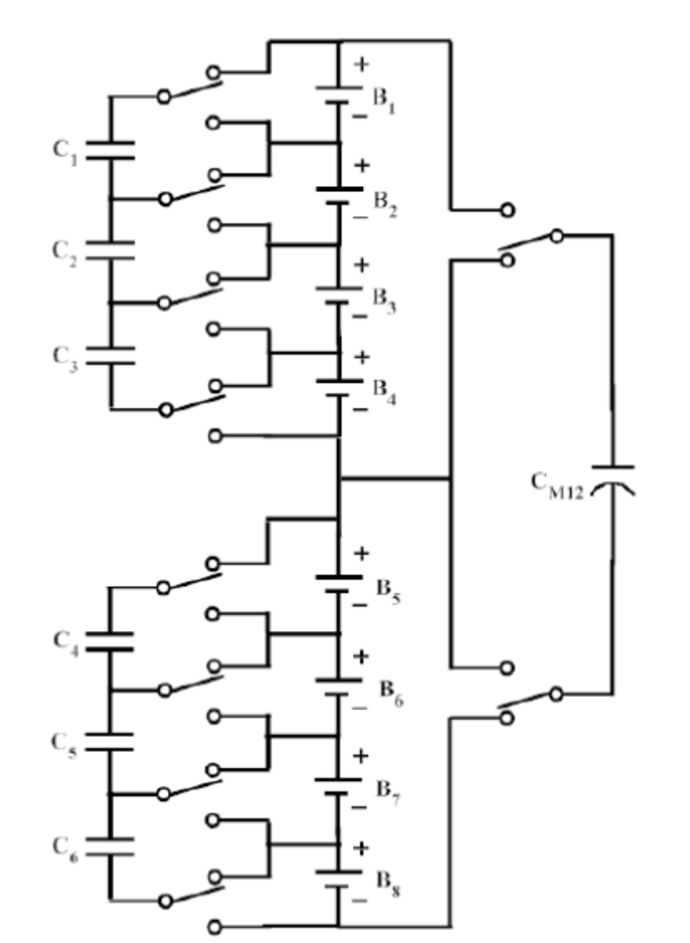
\includegraphics[width=0.6\linewidth]{modulacao_por_baterias}
\caption{Topologias de Equalização com Capacitor Chaveado \cite{energy_figure}}
\label{fig:estrutura_equalizador_passivo_ apacitor}
\end{figure}

 	\newpage
	\thispagestyle{empty}
	\clearpage
	\begin{sidewaysfigure}
		\centering
		\includegraphics[width=1\linewidth]{capa2}
		\label{fig:adc_dac_ideal}
		\caption{Paíneis Solares Concavos \textit{Descrição da Imagem em : Descrições de Capas}}
	\end{sidewaysfigure}
	\clearpage
	%\pagenumbering{gobble}
	\newpage

\section{Ultracapacitores}
Ultra-capacitores são elementos armazenadores de energia que diferem dos
capacitores convencionais apenas no que se refere à tecnologia utilizada para
aproveitar ao máximo as características que confere a esses componentes sua
capacidade armazenadora de cargas. Lembrando que os capacitores armazenam
energia na forma de campo elétrico, sendo este campo provindo de cargas
armazenadas nas porosidades das placas que constituem o mesmo, para elevar a
capacitância do componente basta aumentar a capacidade das placas de
armazenarem cargas em sua superfície, ouatuar modificando a proximidade das
placas, que quanto mais próximas produzem um campo de maior intensidade, e,
culminantemente, uma maior capacitância.Elevando ao máximo essas duas
propriedades pode-se conseguir valores elevados de capacitância, oque foi feito na
aplicação da tecnologia de ultra-capacitores.
A descrição feita anteriormente compara os capacitores com os ultra-caps,
nomenclatura bastante utilizada na literatura, apenas em um aspecto construtivos,
pois de um modo mais descritivo estes diferem bastante. Os capacitores comuns
são nada mais que dois condutores separados por um material não condutor,
enquanto os ultra-capacitores aproximam-se das baterias no que se refere a estes
serem dois eletrodos imersos em um eletrolítico separado por uma membrana
iônica. A Figura 8 abaixo expressa este princípio construtivo[14].

\begin{figure}[h!]
\centering
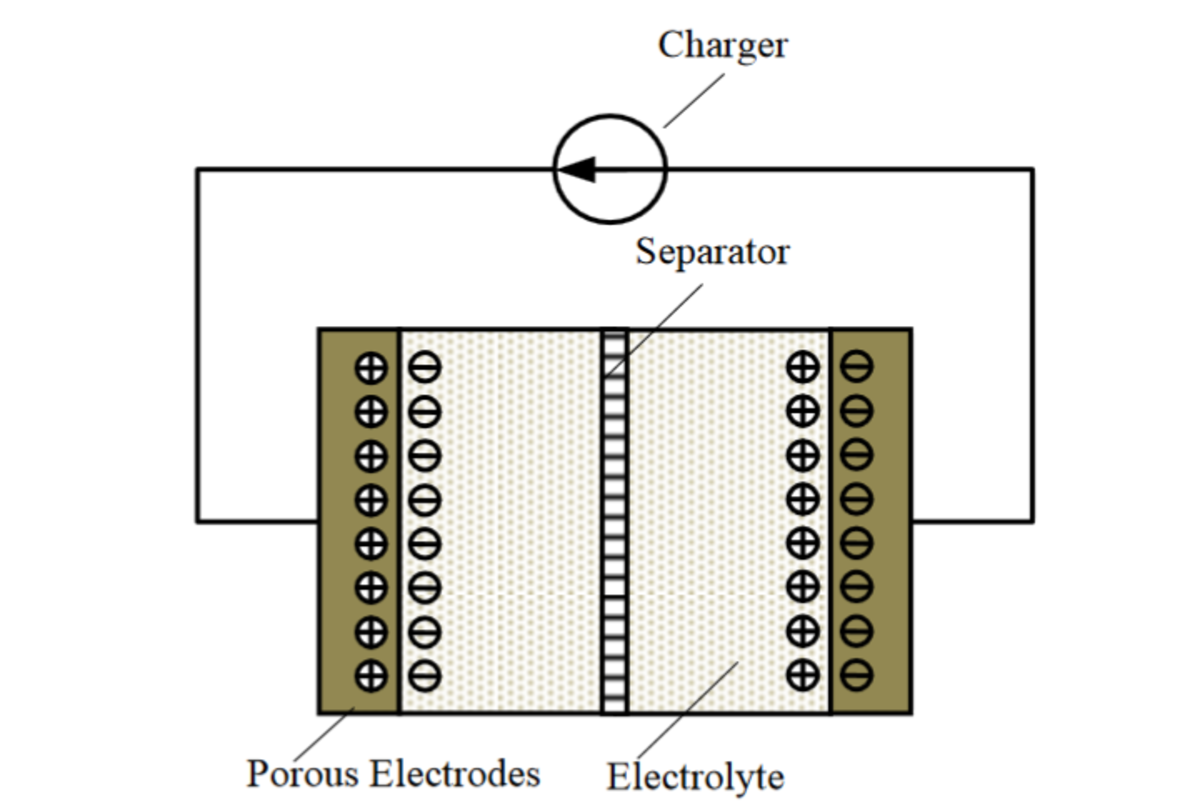
\includegraphics[width=1\linewidth]{Ultracapacitor_interno_construcao}
\caption{Estrutura Double Layer Ultra-Capacitor \cite{ultracapacitor_interno}}
\label{fig:estrutura_equalizador_passivo_ apacitor}
\end{figure}

Os ânions e cátions da solução são atraídos para próximo das placas
positivas e negativas, sem que haja transferência de cargas, como mostra a Figura
8, por meio da estrutura separadora, formando uma fina camada entre os íons e os
eletrodos, sendo análoga a separação entre as placas dos capacitores comuns. O
nome capacitor de dupla camada (Double Layer Capacitor) refere-se a esta
estrutura de duas camadas.\\
Os ultra-capacitores são classificados em diferentes categorias conforme o
material utilizado na construção do eletrodo, sendo os mais comumente utilizados
metais óxidos, carbono e polímeros, bem como a composição do material
eletrolítico, variando entre aquosa, orgânica e polímera.O presente
trabalho não se aprofundará nestes aspectos, pois é de interesse versar sobre o
comportamento destes com relação a um modelo circuital que os represente e não
quanto as tecnologias de engenharia química referentes a sua construção.

\subsection{Modelos Circuitais de Ultracapacitores}
O crescente uso dos ultra-caps trouxe a necessidade prática a que a maior
parte dos sistemas de engenharia estão submetidos: a grande vantagem, ou
necessidade, de simular os efeitos do sistema em questão antes de construí-lo,
evitando o grande desastre de construir algo e que posteriormente não funcione
conforme esperado. Assim, buscou-se desenvolver modelos que representem o
comportamento deste componente em função de outros práticos presentes em
engenharia elétrica, tais como resistências e capacitores comuns, possibilitando
prever o funcionamento do mesmo em seus ciclos de carga e descarga.\\
O valor dos componentes que constituem o modelo equivalente do ultra-cap
em questão varia conforme características do modelo utilizado e segundo os
seguintes aspectos construtivos: resistência do solvente eletrolítico e do material
cujo eletrodo é formado, porosidade da membrana, e qualidade da conexão do
eletrodo-coletor.

\begin{figure}[h!]
\centering
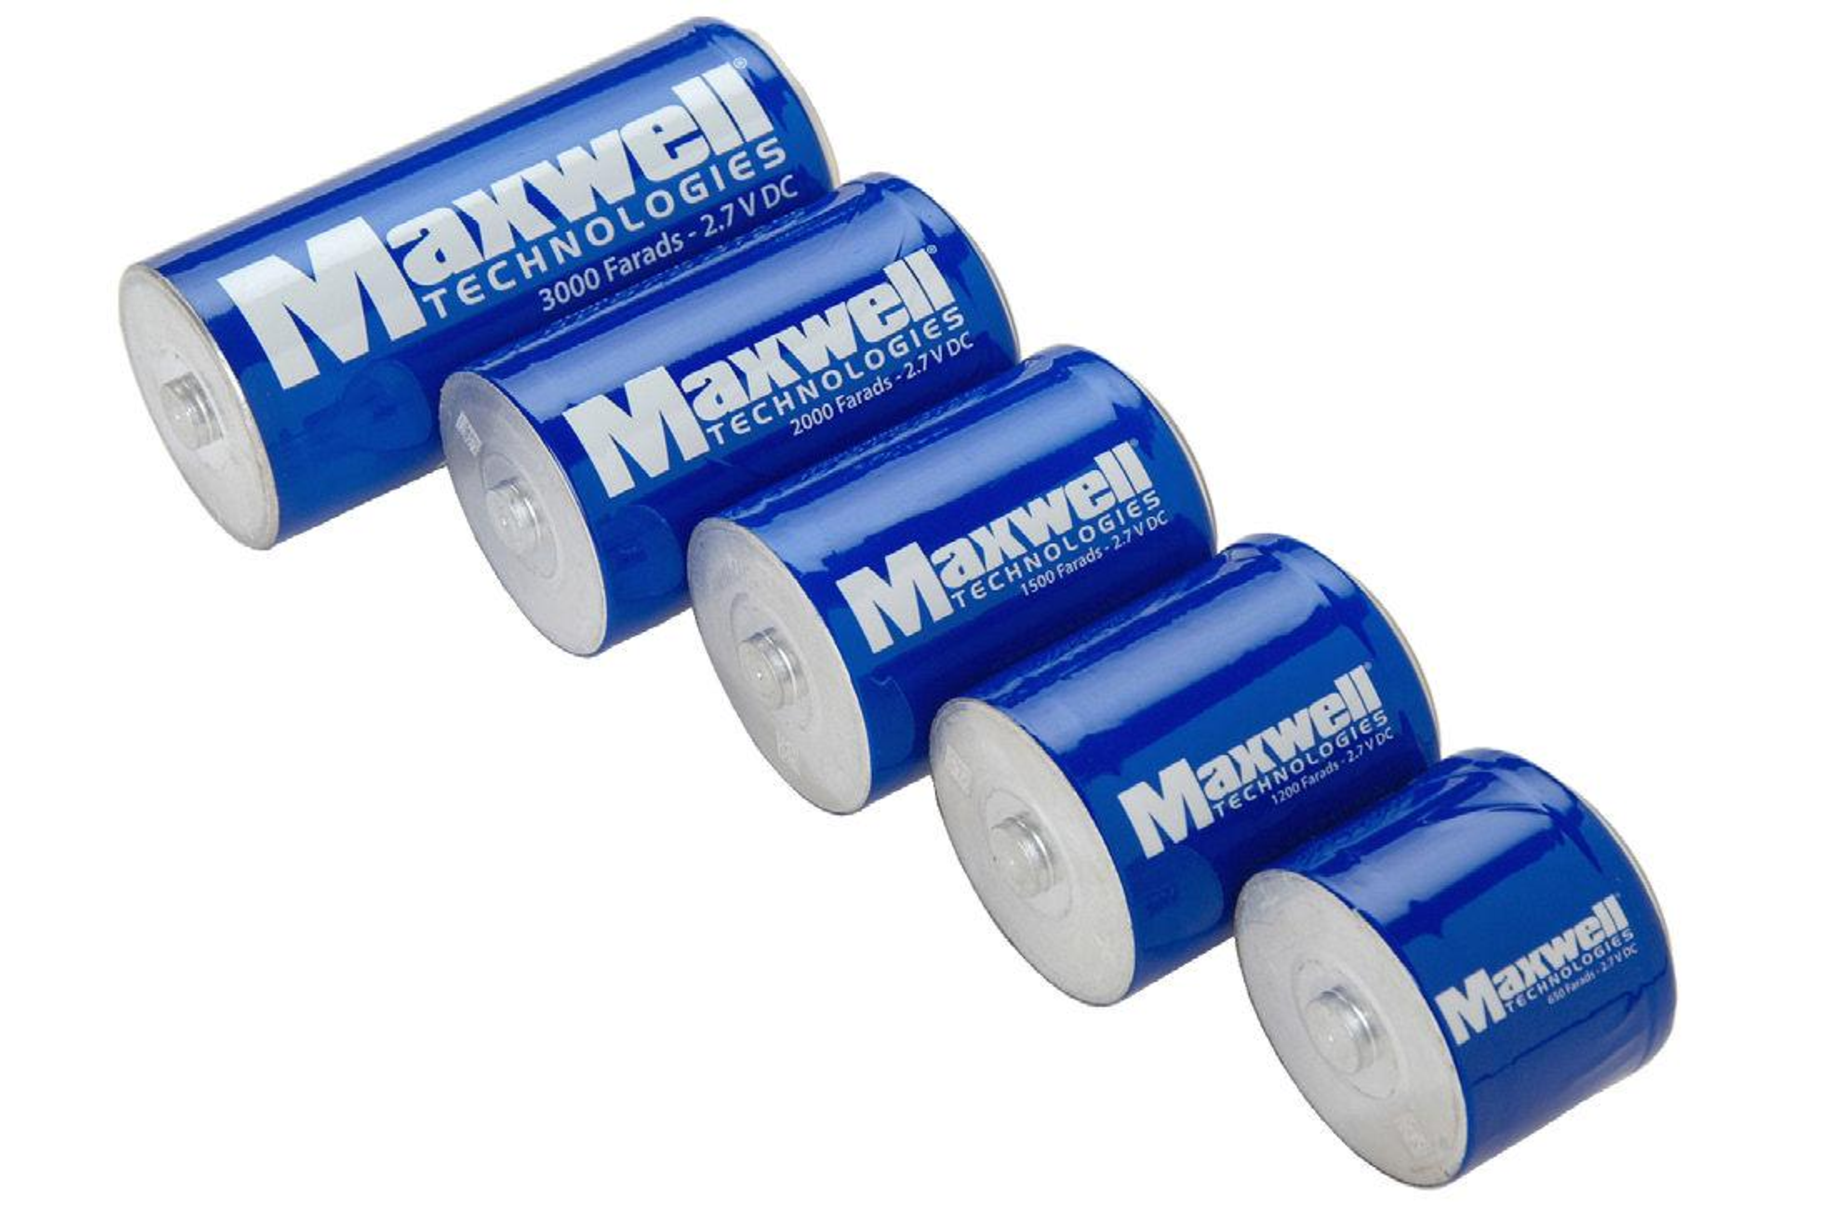
\includegraphics[width=\linewidth]{ultracapacitores}
\caption{Imagem de um Ultracapacitor \cite{ultracapacitor_figura}}
\label{fig:ultracapacitor}
\end{figure}

\newpage

Abaixo, nas Figuras 10 a 13 se encontram alguns modelos circuitais
desenvolvidos para expressar o comportamento de ultra-capacitores DLCs (Double
Layer Capacitor).Os métodos, basicamente, se utilizam de diferente ramos
contendo capacitores e resistências ligados em paralelo com mais combinações
deste tipo. O número destas combinações utilizadas é uma das possíveis formas de
se classificar o modelo utilizado, bem como a devido a presença de capacitâncias
variáveis presentes no circuito.\\
Os valores dos parâmetros presentes nos circuitos simuladores provem da
análise da curva de carregamento do mesmo quando alimentado por uma corrente
constante, porém existem modelos que exigem equipamentos mais sofisticados, tal
como o modelo de linha de transmissão.\\

\begin{figure}[h!]
\centering
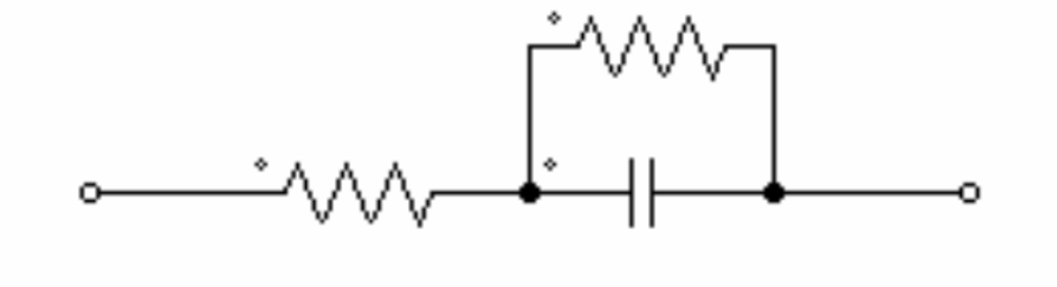
\includegraphics[width=.3\linewidth]{modelo_ultracap_1}
\caption{Modelo Clássico Ultracapcitor \cite{modelo_circuital}}
\label{fig:estrutura_equalizador_passivo_ apacitor}
\end{figure}

\begin{figure}[h!]
\centering
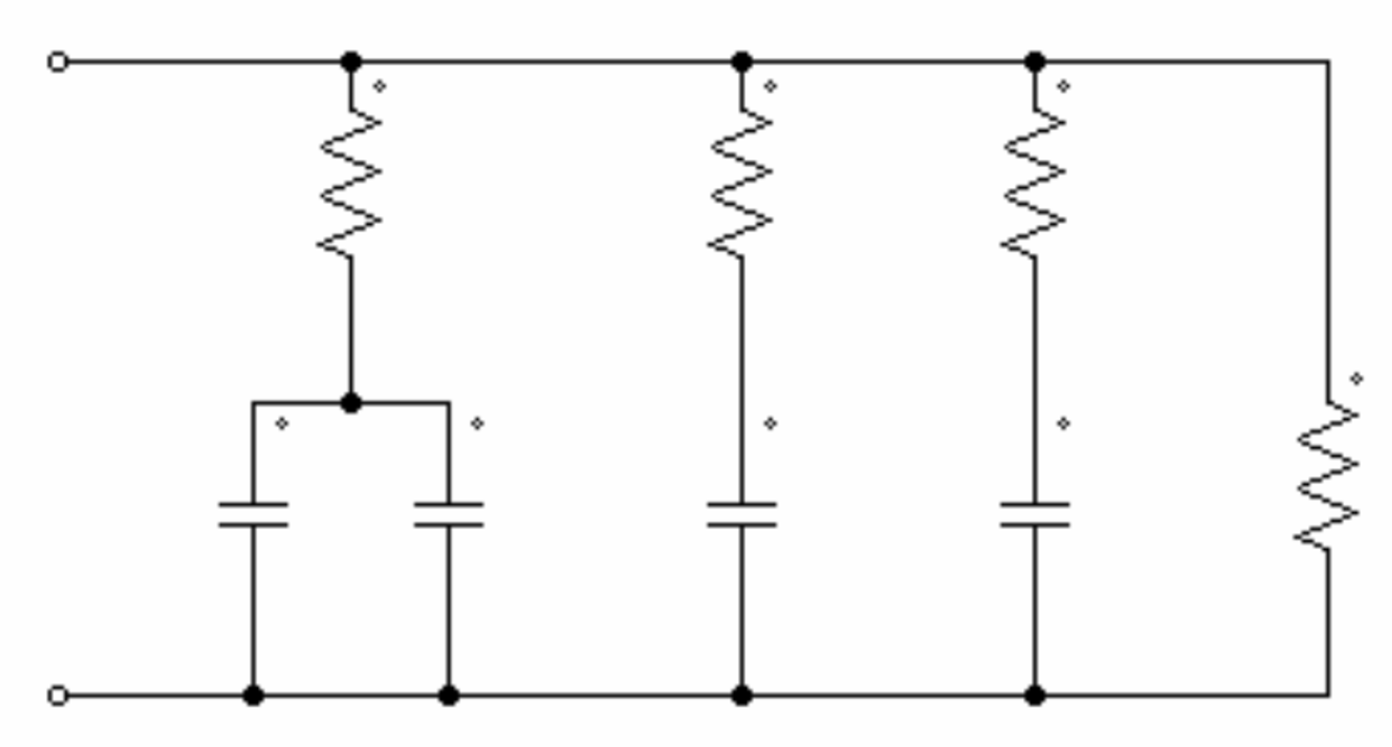
\includegraphics[width=.3\linewidth]{modelo_ultracap_2}
\caption{Modelo Circuital Ultracapacitor Capacitância Variável \cite{modelo_circuital}}
\label{fig:estrutura_equalizador_passivo_ apacitor}
\end{figure}

\begin{figure}[h!]
\centering
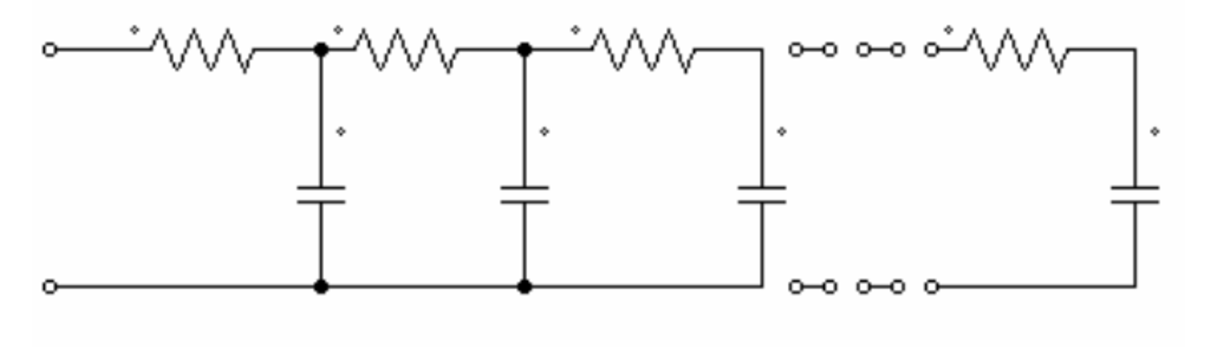
\includegraphics[width=.5\linewidth]{modelo_ultracap_3}
\caption{Modelo Circuital Capacitor de três Ramos \cite{modelo_circuital}}
\label{fig:estrutura_equalizador_passivo_ apacitor}
\end{figure}

Importante destacar que os termos ESR e EPR são siglas para os seguinte
conceitos:equivalent series reistance e equivalentparalelresistance. Tais conceitos
expressam a resistência relacionada a construção do componente, afinal, ao
contrário dos componentes ideais, os utilizados na realidade não possuem
somente características relacionadas a função para o qual foram projetados.Assim,
busca-se representa-los com sendo a característica preponderante em série ou
paralelo com uma resistência, surgindo assim os conceitos de ESR e EPR.
Os circuitos apresentados serão simulados buscando verificar os seus
comportamtentos, bem como procurar o modelo que melhor se encaixe no
comportamento exibido pelo ultra-capacitor utilizado no presente projeto. O
software utilizado para realizar as simulações será o Proteus.

\newpage

 	\newpage
	\thispagestyle{empty}
	\clearpage
	\begin{sidewaysfigure}
		\centering
		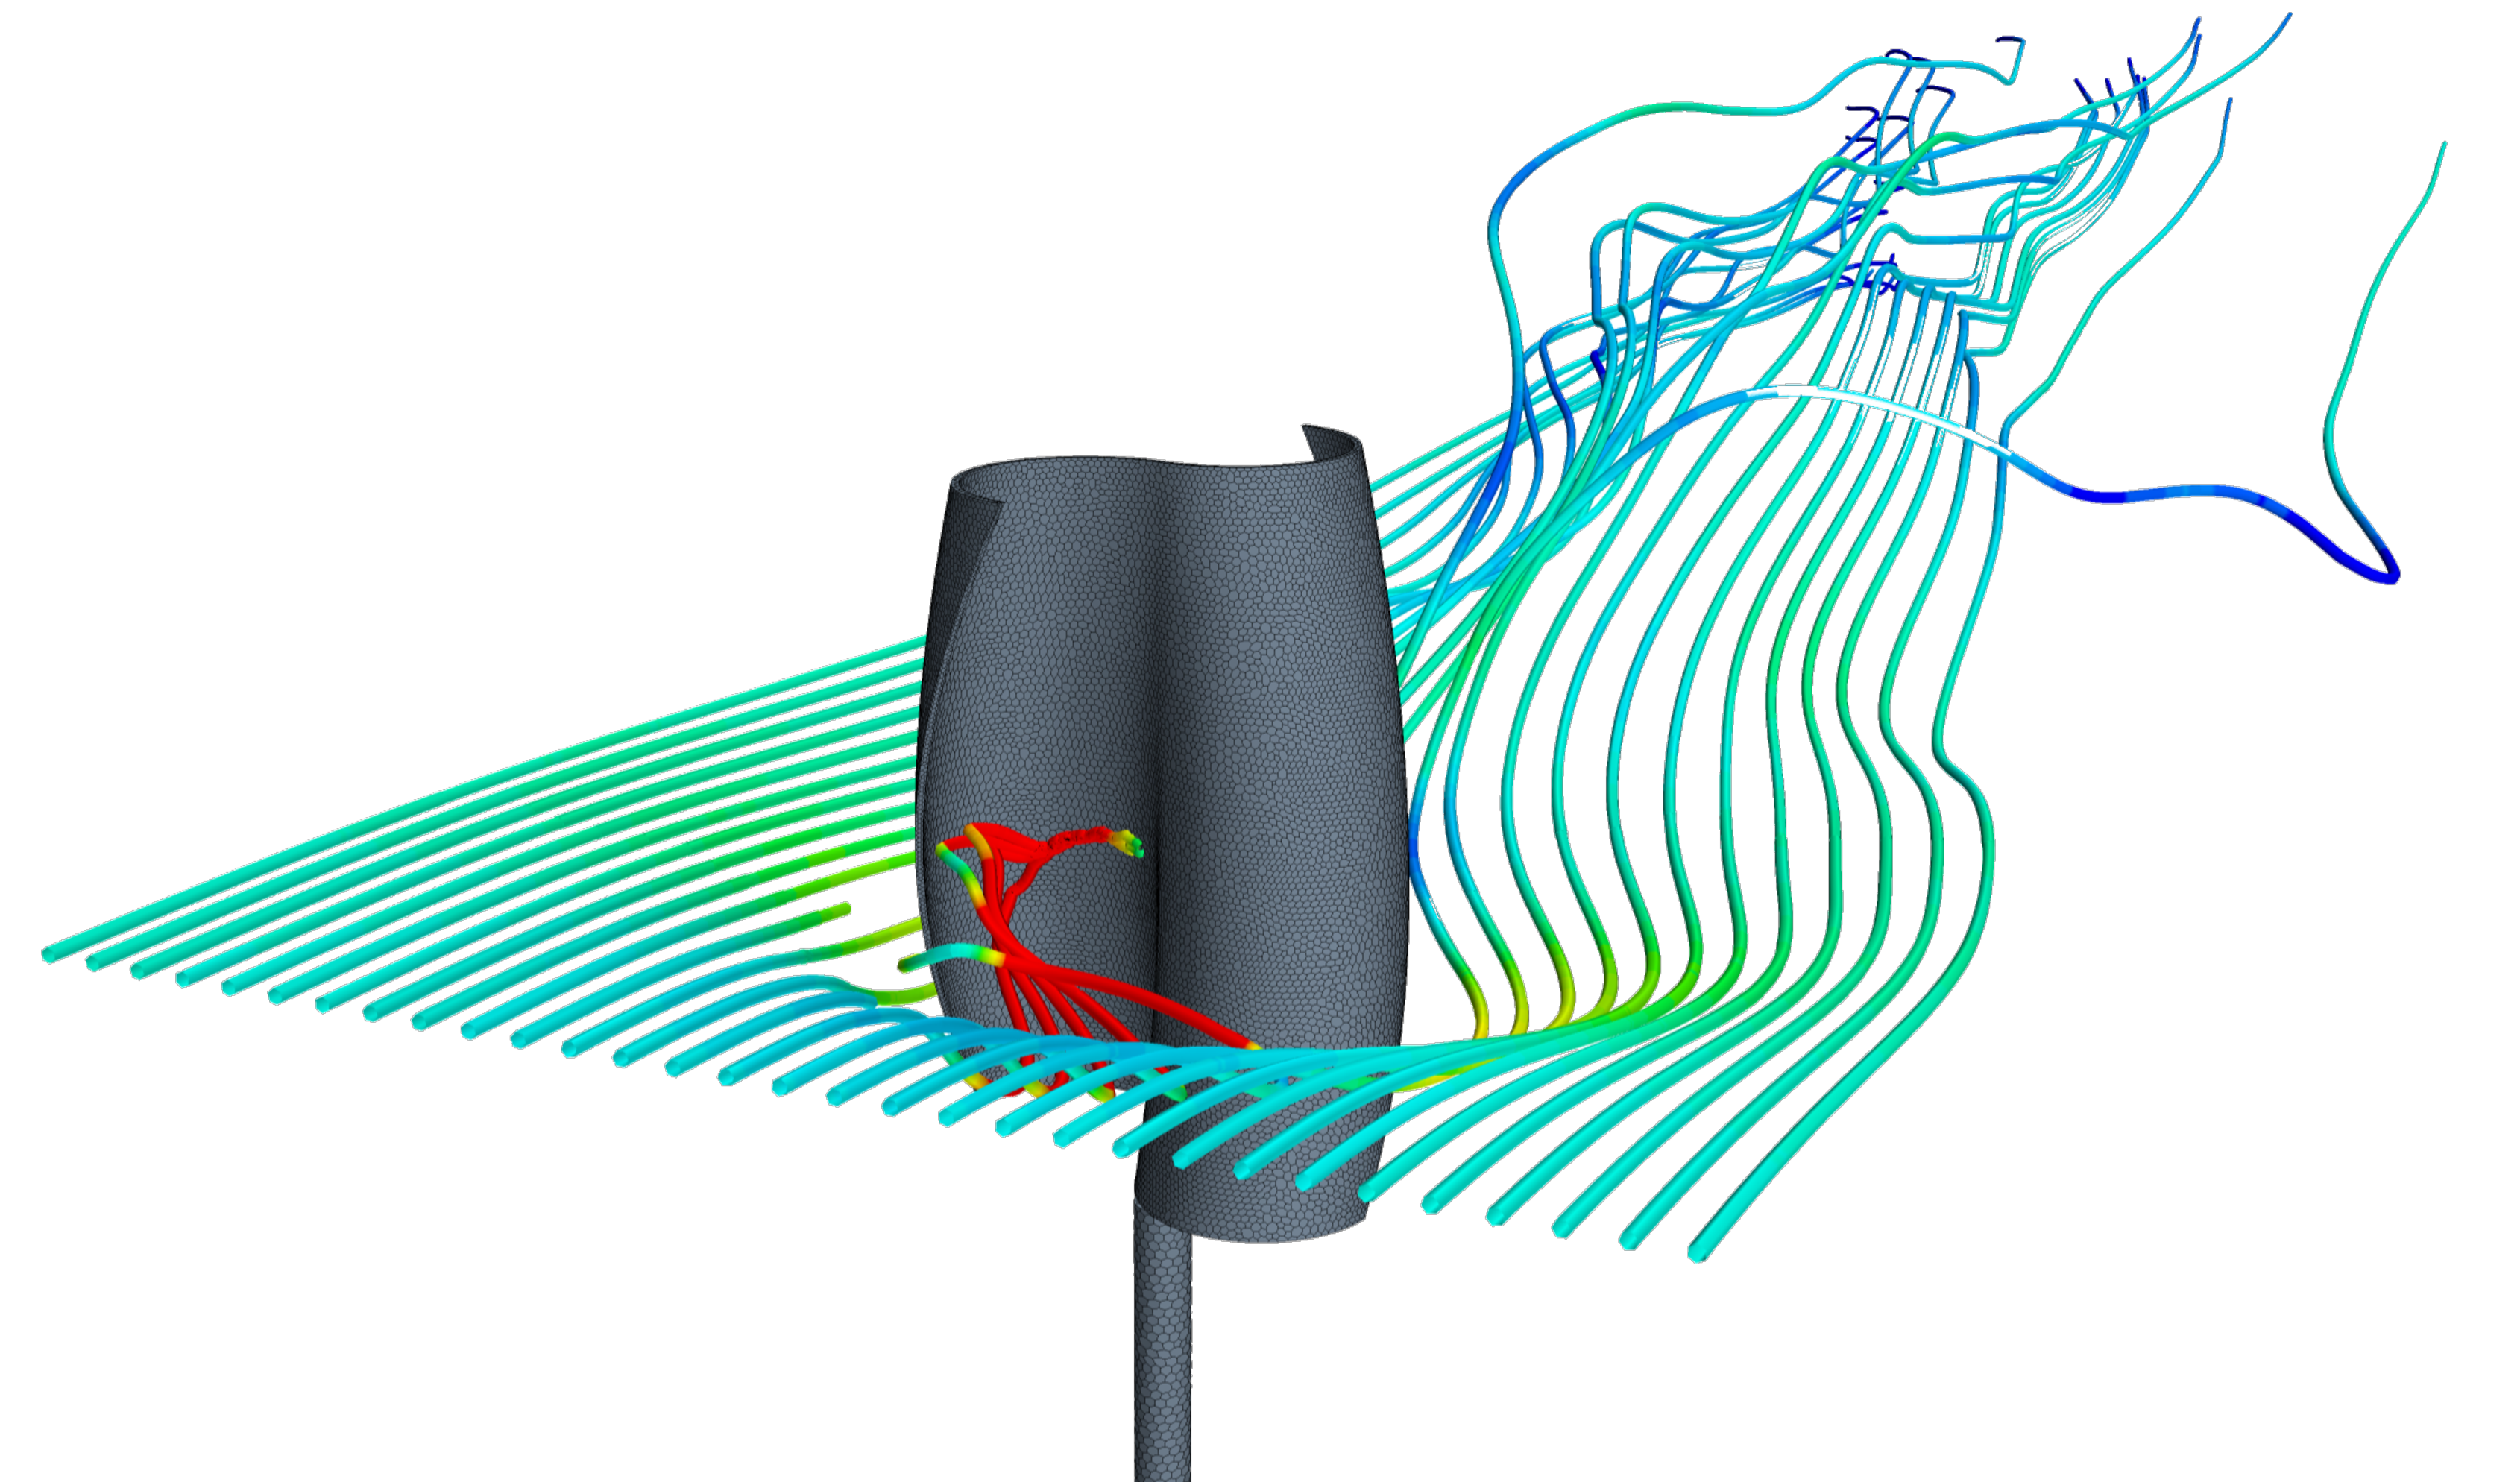
\includegraphics[width=1\linewidth]{capa3}
		\caption{Simulação Fluido Colidindo Com Élice : \textit{Descrição da Imagem em : Descrições de Capas}}
	\end{sidewaysfigure}
	\clearpage
	%\pagenumbering{gobble}
	\newpage
	
\section{Simulações}

\subsection{Topologia Resistor Shunting Não Chaveado}

\begin{figure}[h!]
\centering
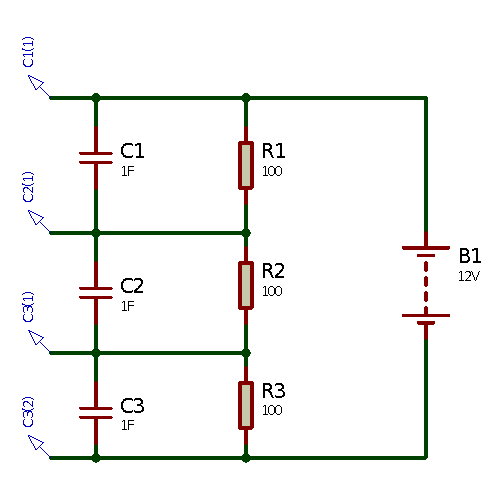
\includegraphics[width=.6\linewidth]{1}
\caption{Circuito Utilizado Para a Simulação \textit{Fonte : Autor}}
\label{fig:estrutura_equalizador_passivo_ apacitor}
\end{figure}

\begin{figure}[h!]
\centering
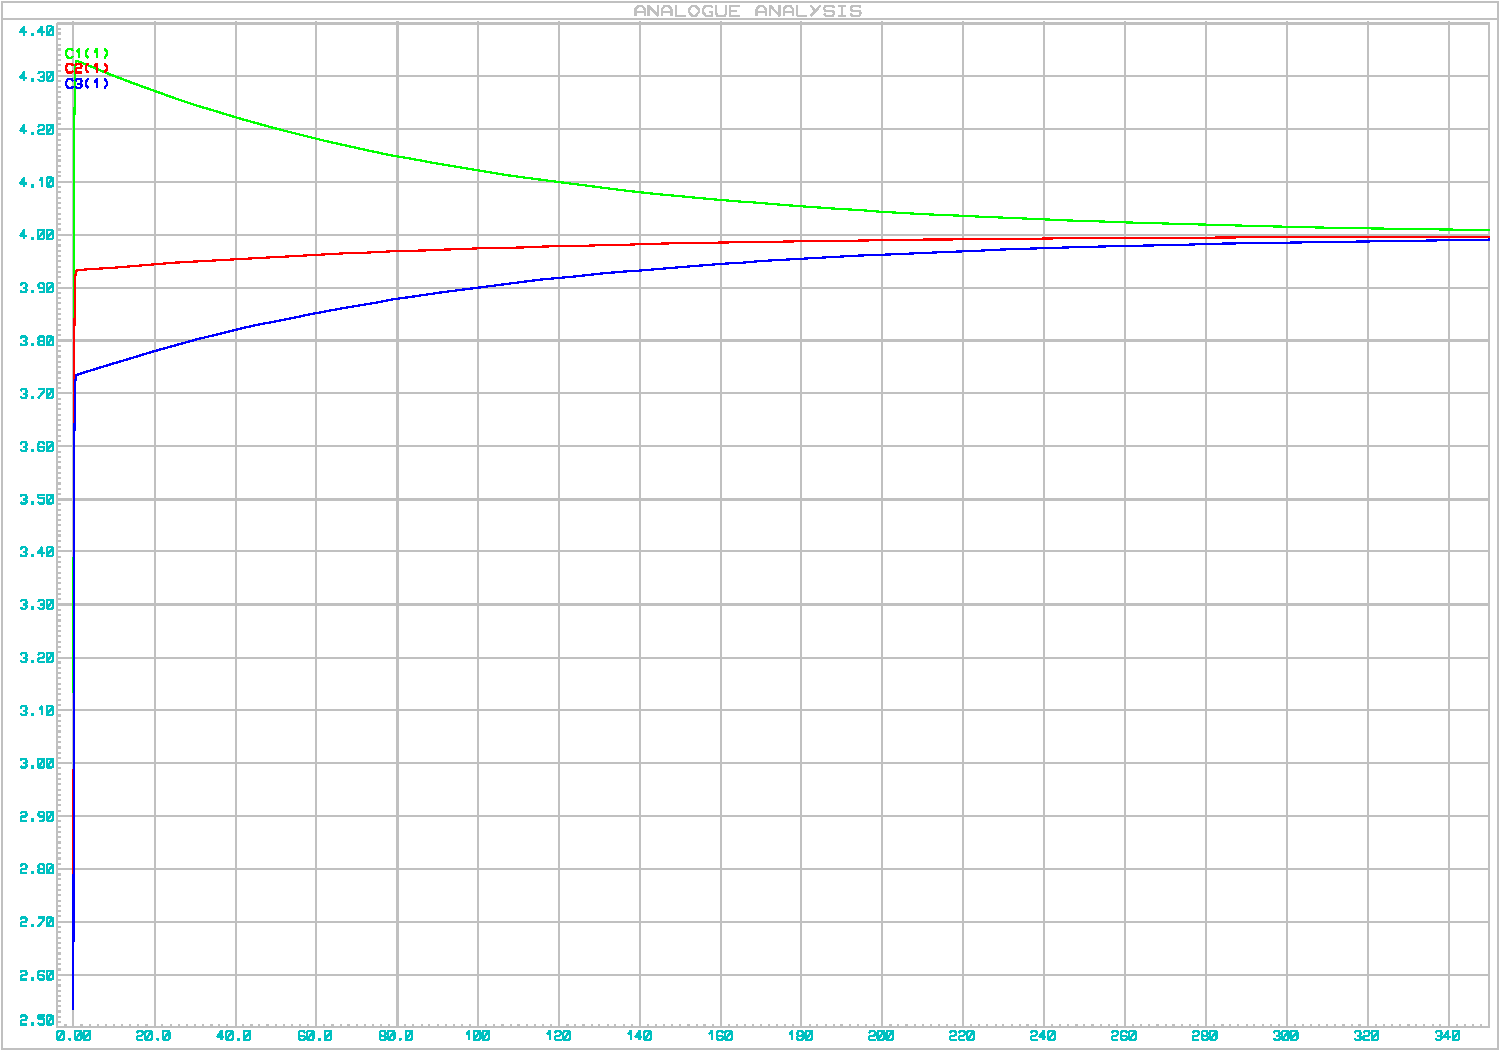
\includegraphics[width=1\linewidth]{Equalizador_de_tensao_ativo_nao_chaveado}
\caption{Simulação Equalização pela Topologia de Ressistor Shunting Ativo Não Chaveado \textit{Fonte : Autor}}
\label{fig:estrutura_equalizador_passivo_ apacitor}
\end{figure}

As linhas representam em cada uma das simulações a diferença de potencial
ao longo de cada célula. Vê-se que inicialmente cada uma das células encontra-se
com um valor diferente de tensão e, conforme o passar do tempo, a tensão tende a
um valor comum, efetuando assim a equalização. Longo tempo de equalização além
do problema relacionado ao consumo de energia são fatores limitadores desta
topologia.

\newpage
\subsection{Topologia Resistor Shunting Chaveado}

\begin{figure}[h!]
\centering
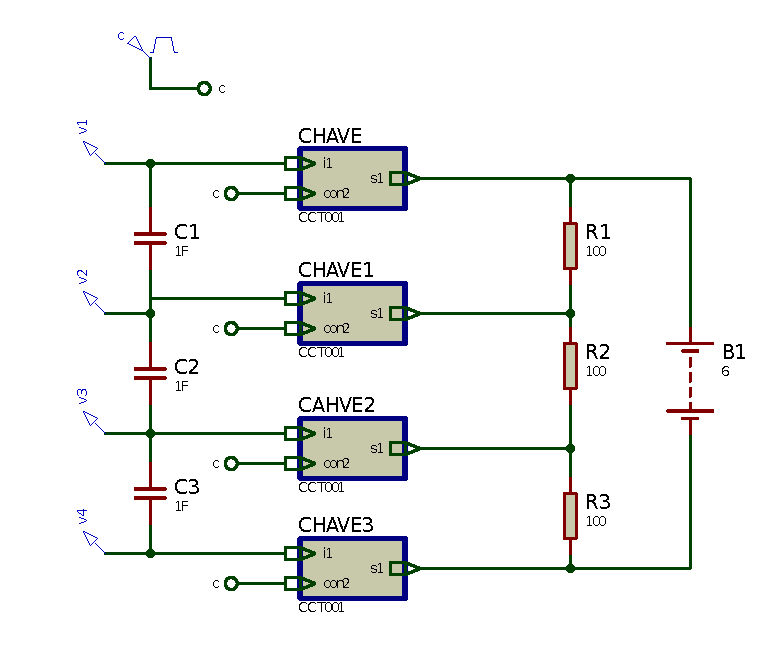
\includegraphics[width=.7\linewidth]{et_1}
\caption{Circuito Utilizado Para a Simulação \textit{Fonte : Autor}}
\label{fig:estrutura_equalizador_passivo_ apacitor}
\end{figure}

\begin{figure}[h!]
\centering
\includegraphics[width=1\linewidth]{ET_ativo_chaveado}
\caption{Simulação Equalização pela Topologia de Ressistor Shunting Ativo Chaveado \textit{Fonte : Autor}}
\label{fig:estrutura_equalizador_passivo_ apacitor}
\end{figure}	

A topologia é a mesma da utilizada com o resistor fixo, porém cada uma das
células é chaveada durante o processo. Problemas relacionados ao longo tempo de
equalização e ao consumo de energia, assim como no caso do resistor fixo, são
problemas relacionados a esta topologia.

\newpage

\subsection{Capacitor Chaveado}

\begin{figure}[h!]
\centering
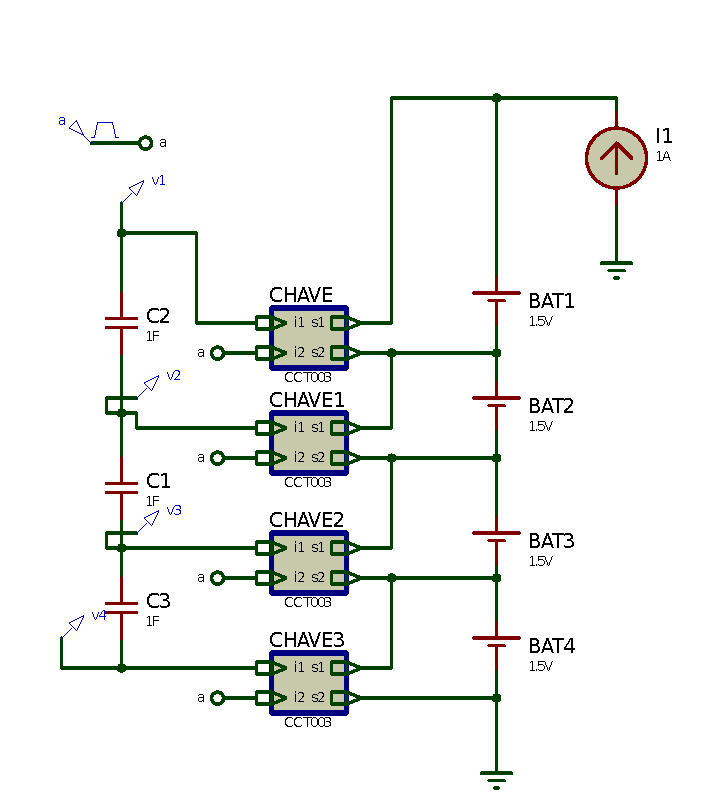
\includegraphics[width=1\linewidth]{Equalizador_de_tensao_chaveado}
\caption{Simulação Equalização pela Topologia de Ressistor Shunting Ativo Não Chaveado \textit{Fonte : Autor}}
\label{fig:estrutura_equalizador_passivo_ apacitor}
\end{figure}

\begin{figure}[h!]
\centering
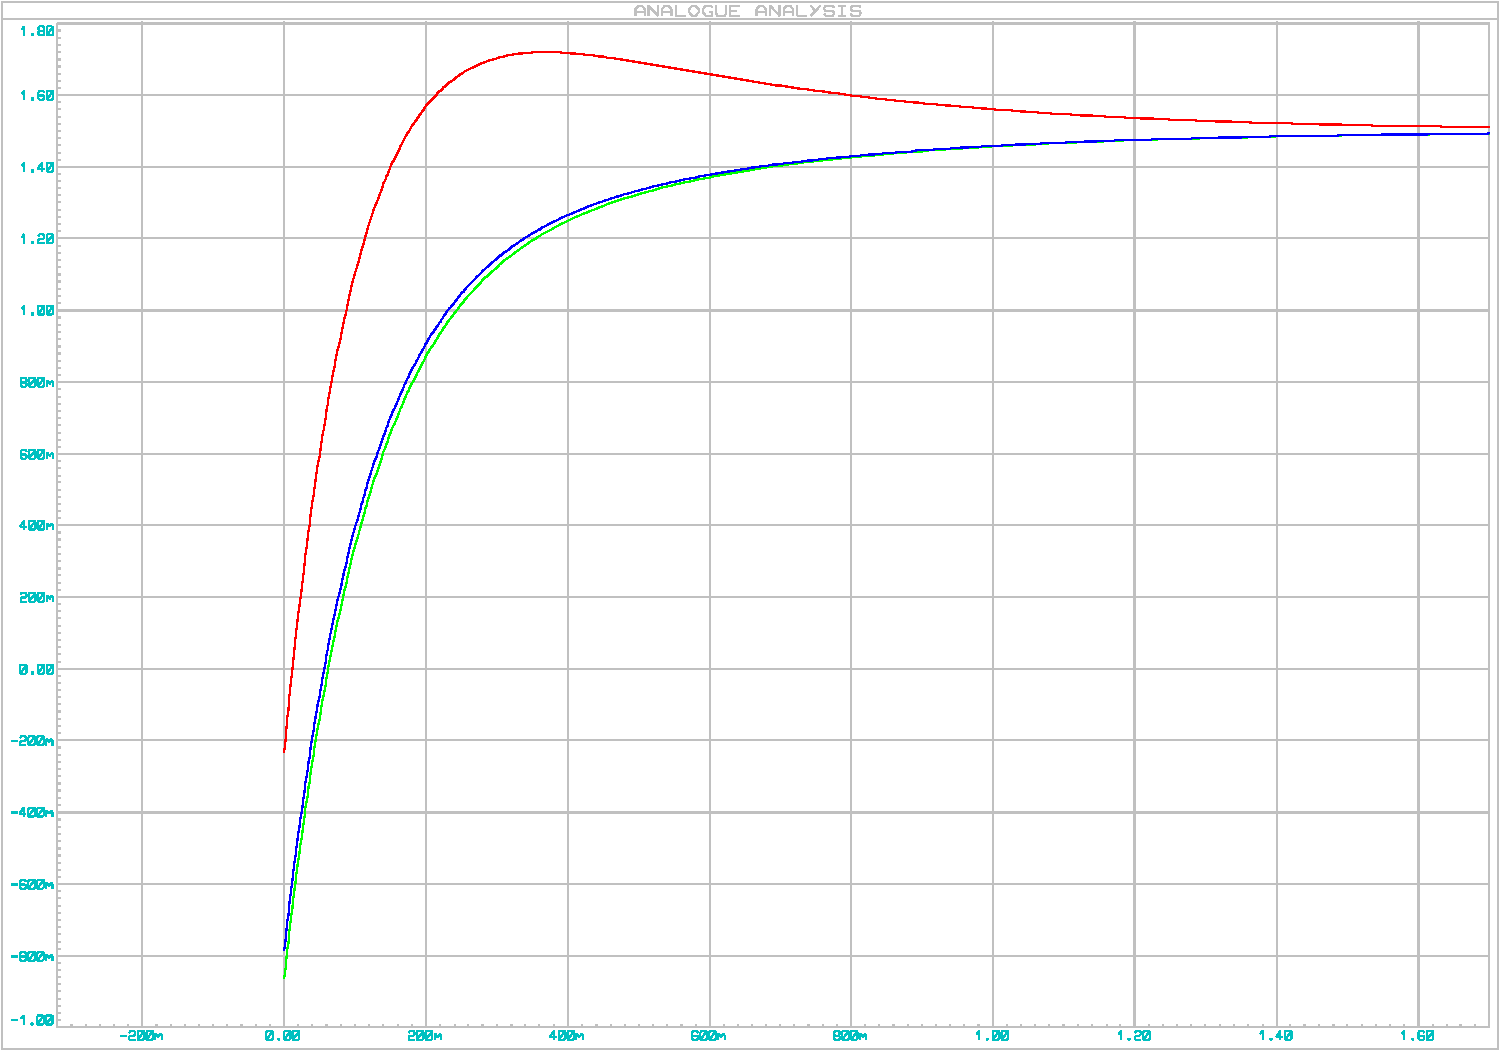
\includegraphics[width=1\linewidth]{Equalizador_de_te_sao_chaveado}
\caption{Simulação Equalização pela Topologia de Capacitores Como Elementos Transportadores de Energia \textit{Fonte : Autor}}
\label{fig:estrutura_equalizador_passivo_ apacitor}
\end{figure}

Esta topologia utiliza capacitores como elemento que direciona o excesso de
energia de uma célula para outra, culminando no fato de que não há consumo de
parte alguma da energia armazenada, sendo uma característica bastante vantajosa
das topologias passivas. As linhas mostram que no regime permanente a tensão ao
longo das células é a mesma.

\newpage

\subsection{Capacitor Único Chaveado}

\begin{figure}[h!]
\centering
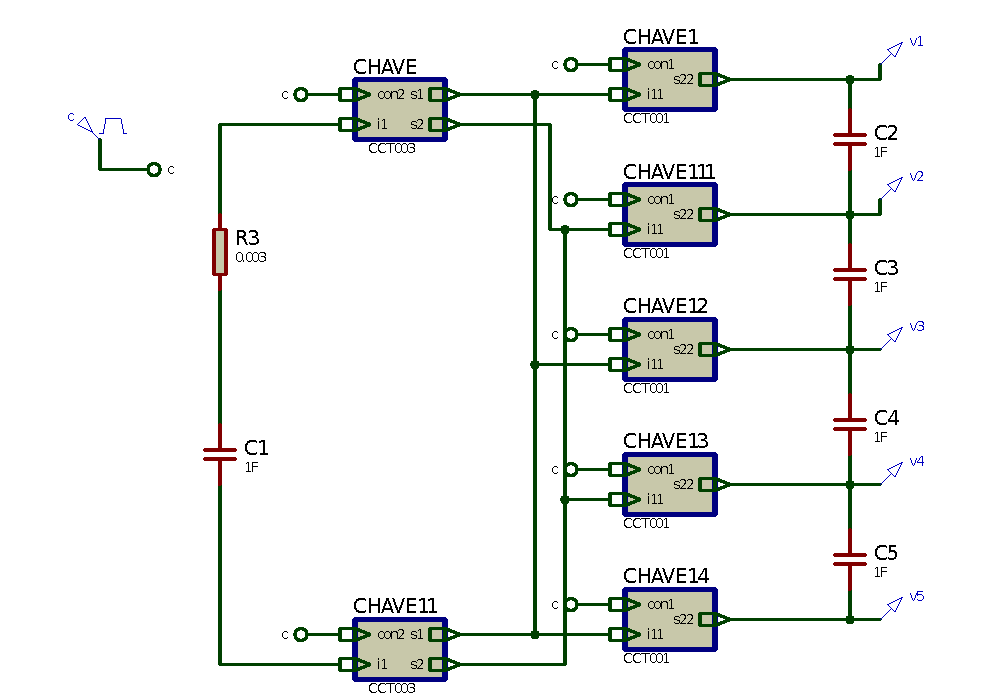
\includegraphics[width=1\linewidth]{ETCC1}
\caption{Simulação Equalização pela Topologia de Capacitores Como Elementos Transportadores de Energia \textit{Fonte : Autor}}
\label{fig:estrutura_equalizador_passivo_ apacitor}
\end{figure}

\begin{figure}[h!]
\centering
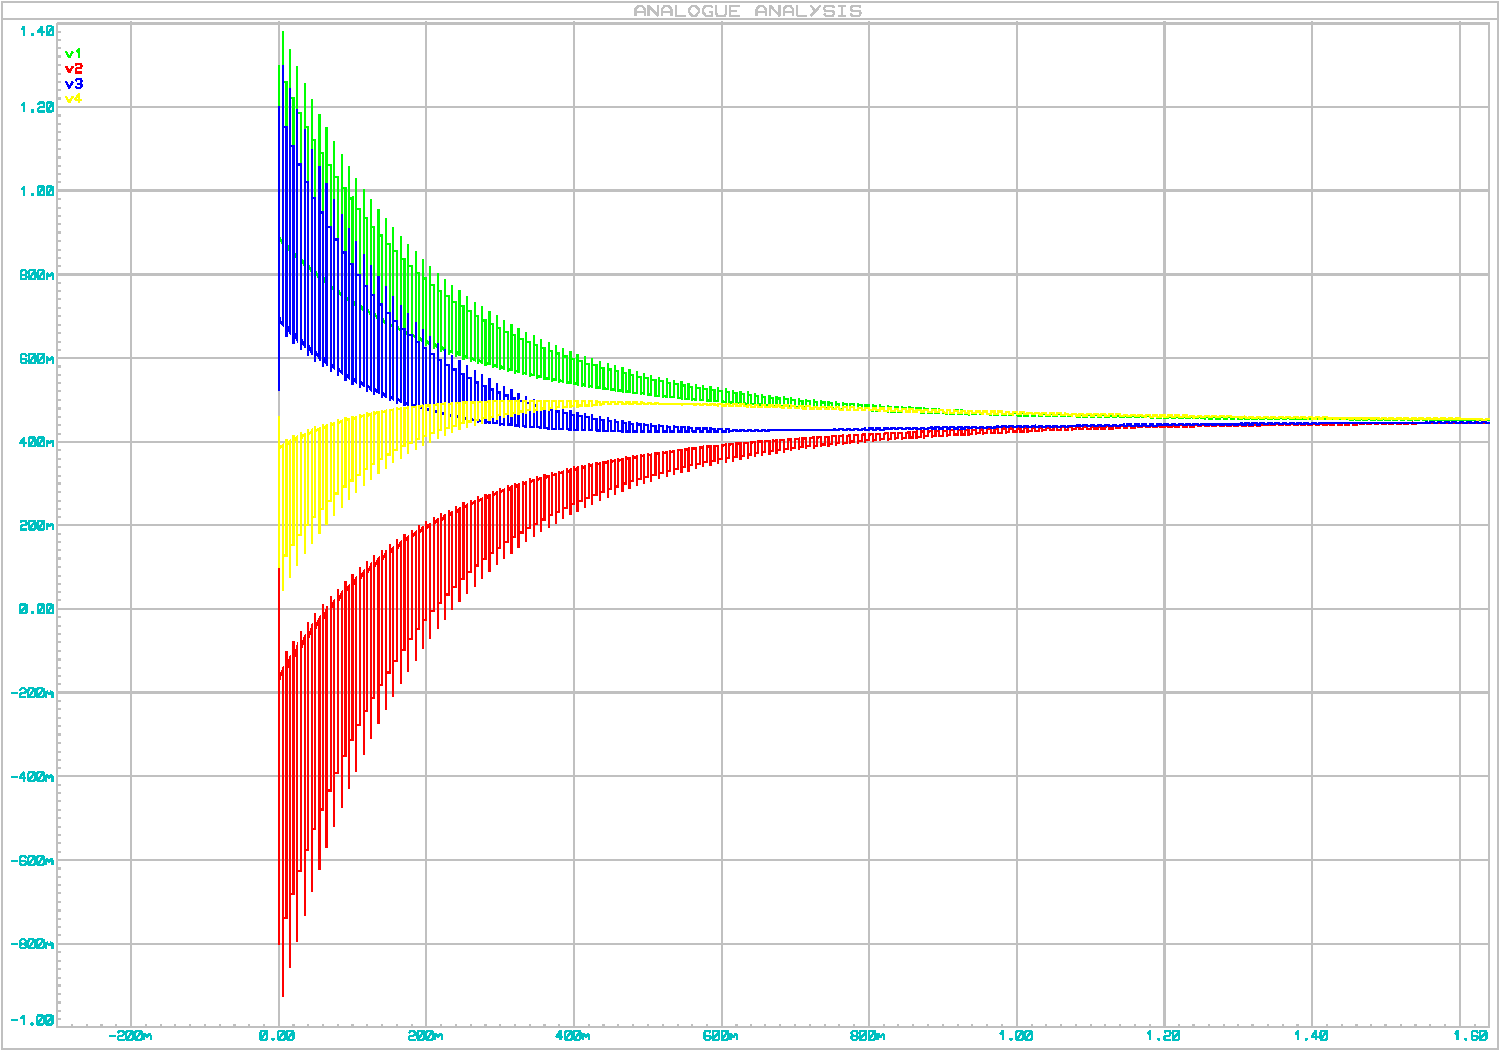
\includegraphics[width=.8\linewidth]{etcc}
\caption{Simulação Equalização pela Topologia de Capacitores Como Elementos Transportadores de Energia \textit{Fonte : Autor}}
\label{fig:estrutura_equalizador_passivo_ apacitor}
\end{figure}

Esta topologia, também passiva, também utiliza capacitores como elemento
que direciona a energia de uma célula para outra, porém agora o método é
chaveado. As curvas indicam que em regime estacionário a tensão ao longo das
células tende a um mesmo valor.

\newpage

\subsection{Capacitor Duplo Chaveado}

\begin{figure}[h!]
\centering
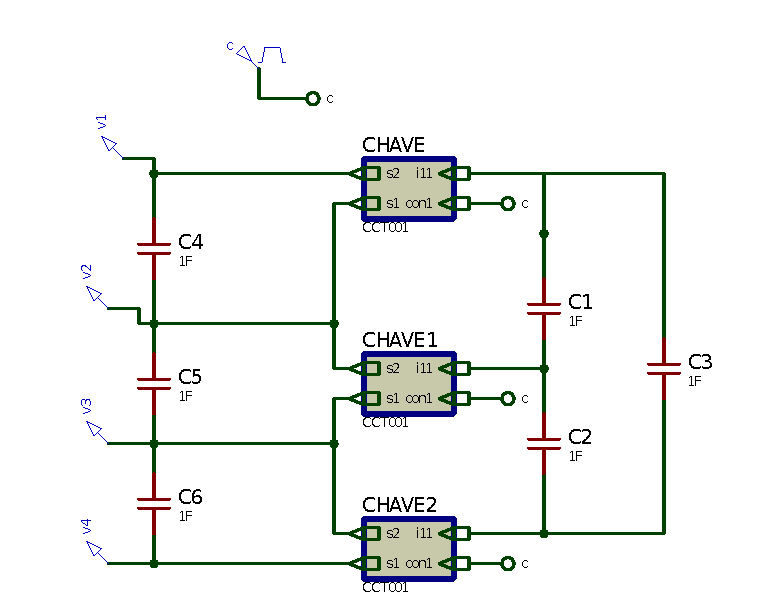
\includegraphics[width=1\linewidth]{etc_3_capacitor}
\caption{Simulação Equalização pela Topologia de três Capacitores \textit{Fonte : Autor}}
\label{fig:estrutura_equalizador_passivo_ apacitor}
\end{figure}

\begin{figure}[h!]
\centering
\includegraphics[width=1\linewidth]{tres_capacitores}
\caption{Simulação Equalização pela Topologia de três Capacitores \textit{Fonte : Autor}}
\label{fig:estrutura_equalizador_passivo_ apacitor}
\end{figure}

Esta topologia também utiliza capacitores como elemento que transfere
energia entre as células. As curvas mostram que a tensão ao fim do processo é a
mesma em cada célula. O fato desta equalização ser passiva é uma vantagem,
porém o grande número de capacitores utilizados é uma das limitações, afinal são
dois por célula.

\newpage

\subsection{Modulação Por Baterias}

\begin{figure}[h!]
\centering
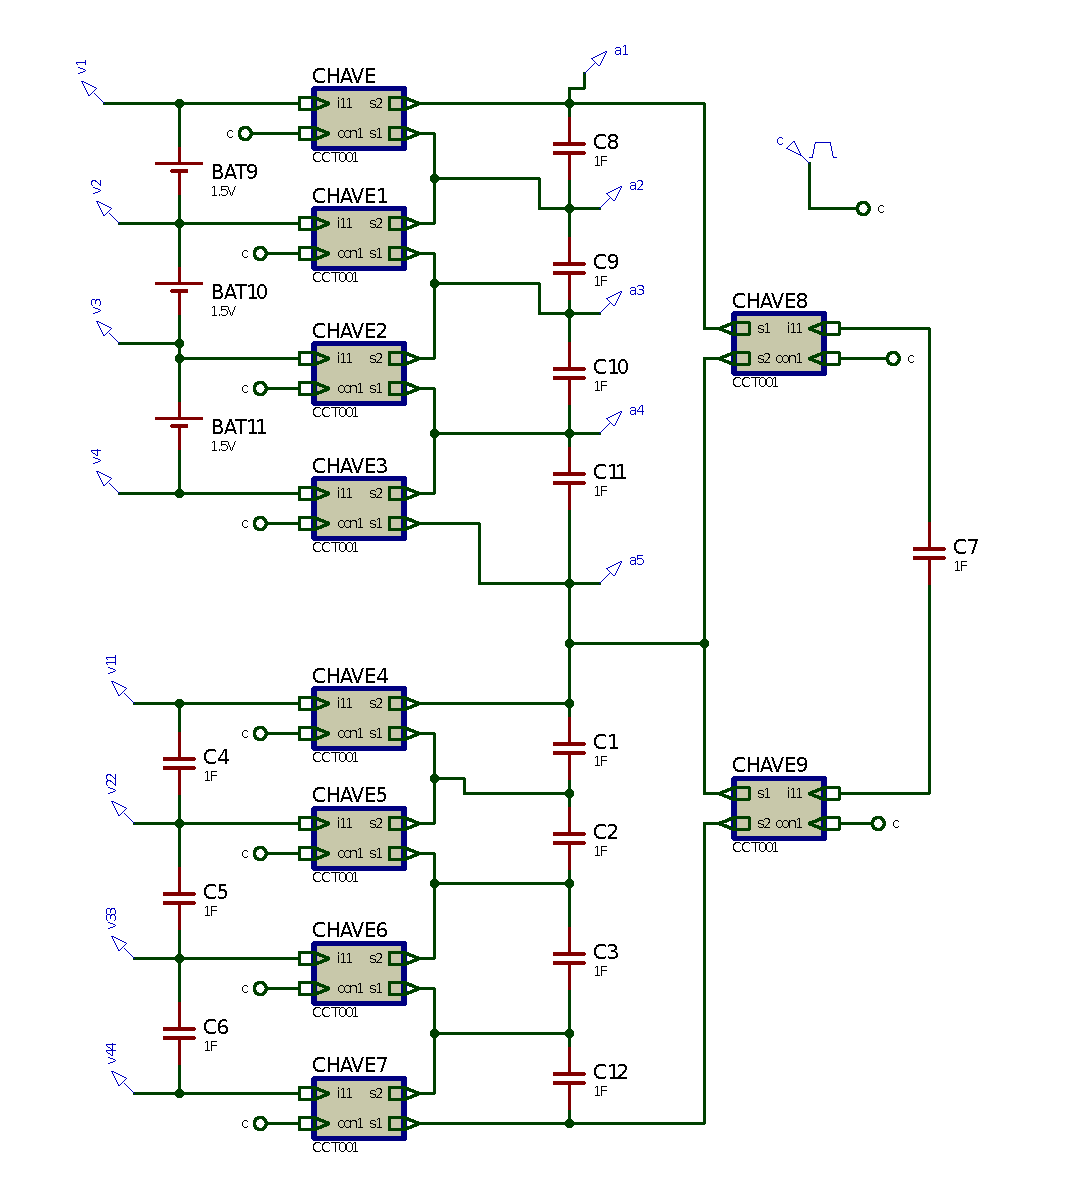
\includegraphics[width=1\linewidth]{ETC_Diversos_capacitores}
\caption{Simulação Equalização pela Topologia de três Capacitores \textit{Fonte : Autor}}
\label{fig:estrutura_equalizador_passivo_ apacitor}
\end{figure}

\begin{figure}[h!]
\centering
\includegraphics[width=1\linewidth]{diversos_capacitores}
\caption{Simulação Equalização pela Topologia de três Capacitores \textit{Fonte : Autor}}
\label{fig:estrutura_equalizador_passivo_ apacitor}
\end{figure}

Esta topologia utiliza baterias como elemento que transfere a energia de
uma célula para outra, sendo uma topologia passiva de equalização. Os módulos
formados pelas baterias são sub-dividos em módulos internos que auxiliam na
equalização. A quantidade de elementos utilizados para a construção do
equipamento é um dos fatores negativos desta topologia.

 	\newpage
	\thispagestyle{empty}
	\clearpage
	\begin{sidewaysfigure}
		\centering
		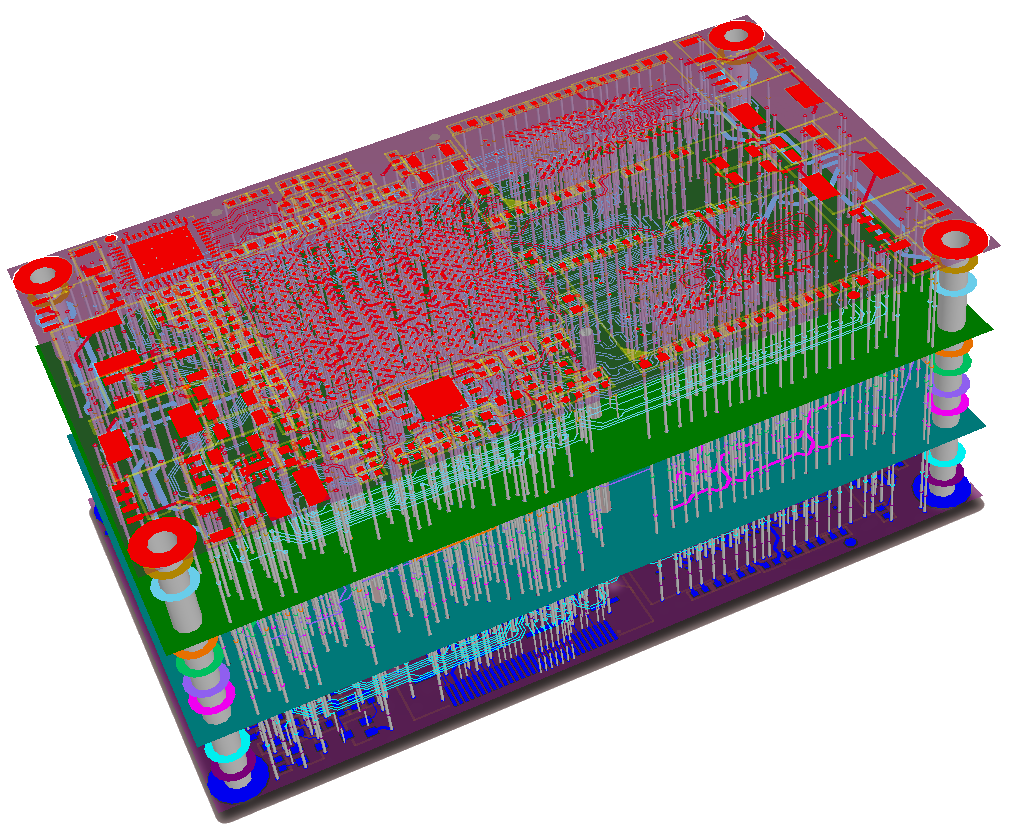
\includegraphics[width=1\linewidth]{capa5.png}
		\caption{Abstração do Roteamento de Placas \textit{Descrição da Imagem em : Descrições de Capas}}
		\label{fig:adc_dac_ideal}
	\end{sidewaysfigure}
	\clearpage
	%\pagenumbering{gobble}
	\newpage
	
\section{Construção e Análise do Equalizador de Tensão Proposto no Presente Trabalho}
A topologia escolhida para equalizar o banco de ultra-caps utilizado na
presente pesquisa consiste em um modelo chaveado que permite a passagem de
cargas das células mais carregadas para as menos conforme é verificada uma
diferença de potencial entre elas. O componente utilizado para realizar a
verificação desta diferença de potencial entre as células é um amplificador
operacional comparador de baixa tensão, adequado aos padrões de tensão de
funcionamento dos ultra-caps, que é por volta de 2.7 volts. A figuras (\ref{fig:topologia_dos_equlizadores_utilizados_no_presente_trabalho})
expressam as topologias a serem utilizadas, cuja característica determinante
para diferenciá-las é a corrente de equalização permitida que pode assumir valores
de 10mA e 300mA. Ambas os circuitos encontram-se nas figuras abaixo,
juntamente com a topologia proposta.

\begin{figure}[h!]
\centering
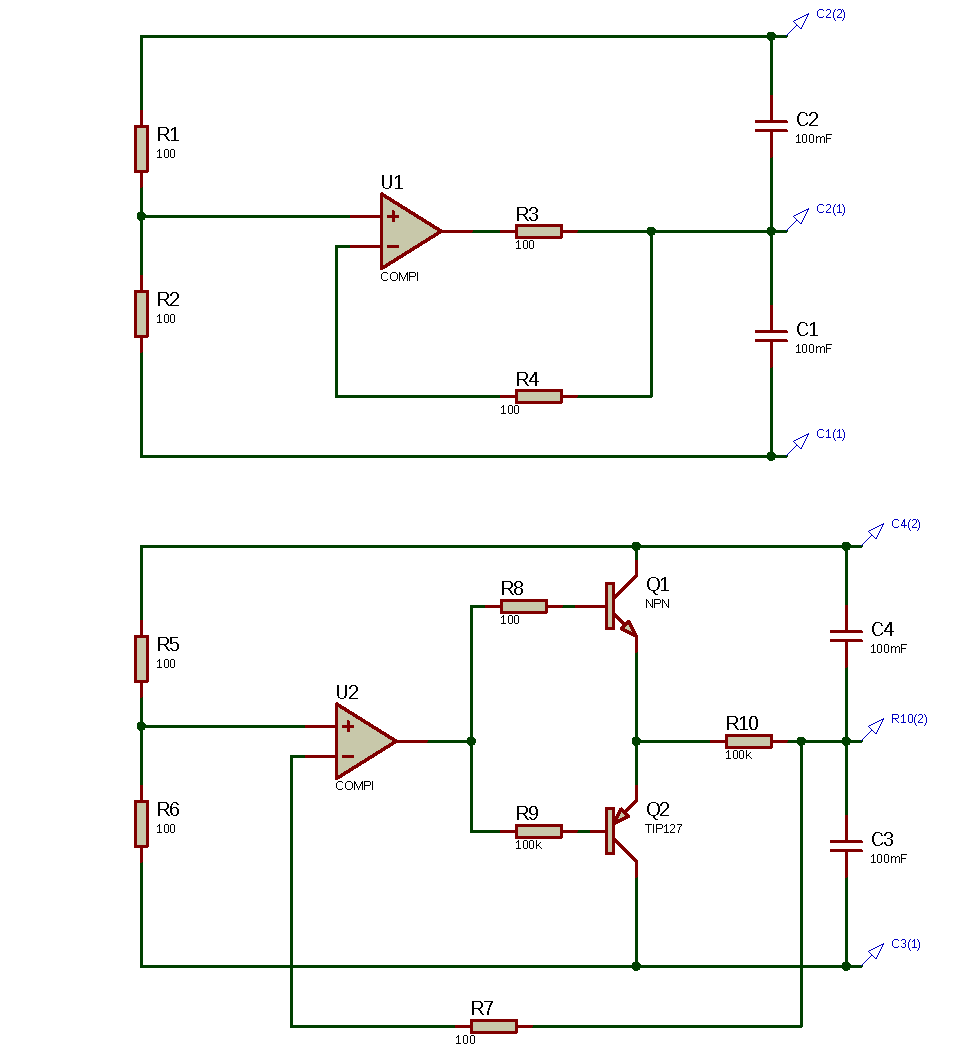
\includegraphics[width=0.9\linewidth]{topologias_equalizadoras_de_100e_10ma}
\caption{Topologias de 100 e 300mA \textit{Fonte : Autor}}
\label{fig:topologia_dos_equlizadores_utilizados_no_presente_trabalho}
\end{figure}

\begin{figure}[h!]
\centering
\includegraphics[width=0.9\linewidth]{simulacao_topologia_10ma_300ma}
\caption{Simulação das Topologias de 100 e 300mA \textit{Fonte : Autor}}
\label{fig:topologia_dos_equlizadores_utilizados_no_presente_trabalho}
\end{figure}

\newpage

A simulação das topologias apresentadas acima encontra-se abaixo e
apresenta-se em conformidade com o comportamento esperado. A diferença de
potencial em cada célula tende a um valor e igual em ambas, sendo exatamente
esta a função do circuito equalizador

\subsection{Construção do Componente}
A estrutura equalizadora se encaixa nas células ultra-capacitivas, devido a
isto suas dimensões dependem da distância entre os capacitores e, como
consequência, da forma como serão ligados os ultra-caps para formar o banco
capacitivo. Por esta razão ainda não foi decidido quais as dimensões do
componente, porém tais informações podem diferir bruscamente do apresentado
parcialmente neste relatório. A confecção do projeto foi feita por meio do software
\textit{Proteus}.\\
Tendo em mão o circuito simulado e funcionando de um modo próximo ao
esperado, afinal as simulações expressam valores distintos, porém buscam um
ponto de equalização comum, cabe agora confeccionar o dispositivo.Como foi dito,
as dimensões e formato do mesmo dependem de como será montada a caixa
contendo os ultra-capacitores. Abaixo encontram-se imagens expressando
possíveis modos de se organizar ultra-capacitores, implicando na modificação do
formato do equalizador de tensão.Uma das imagens mostra um sistema de
equalização montado sobre uma placa aonde encaixam-se os ultra-caps, sendo uma
possibilidade de construção dos dispositivo.

\begin{figure}[h!]
\centering
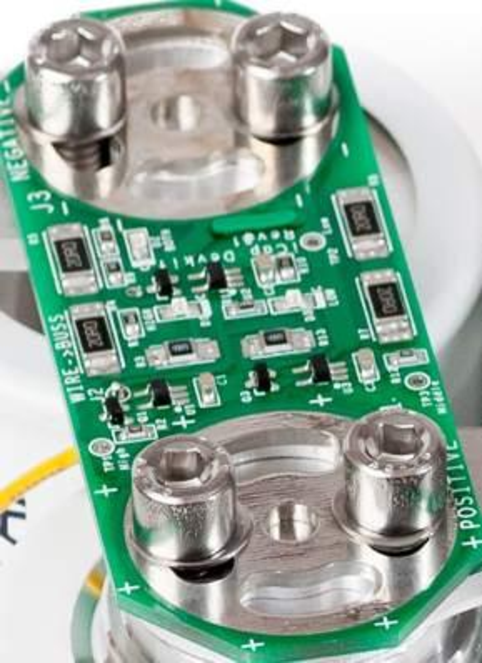
\includegraphics[width=0.55\linewidth]{equlizador_de_tensao}
\caption{Equalizador de Tensão Próximo ao Proposto no Presente Documento}
\label{fig:topologia_dos_equlizadores_utilizados_no_presente_trabalho}
\end{figure}

\begin{figure}[h!]
\centering
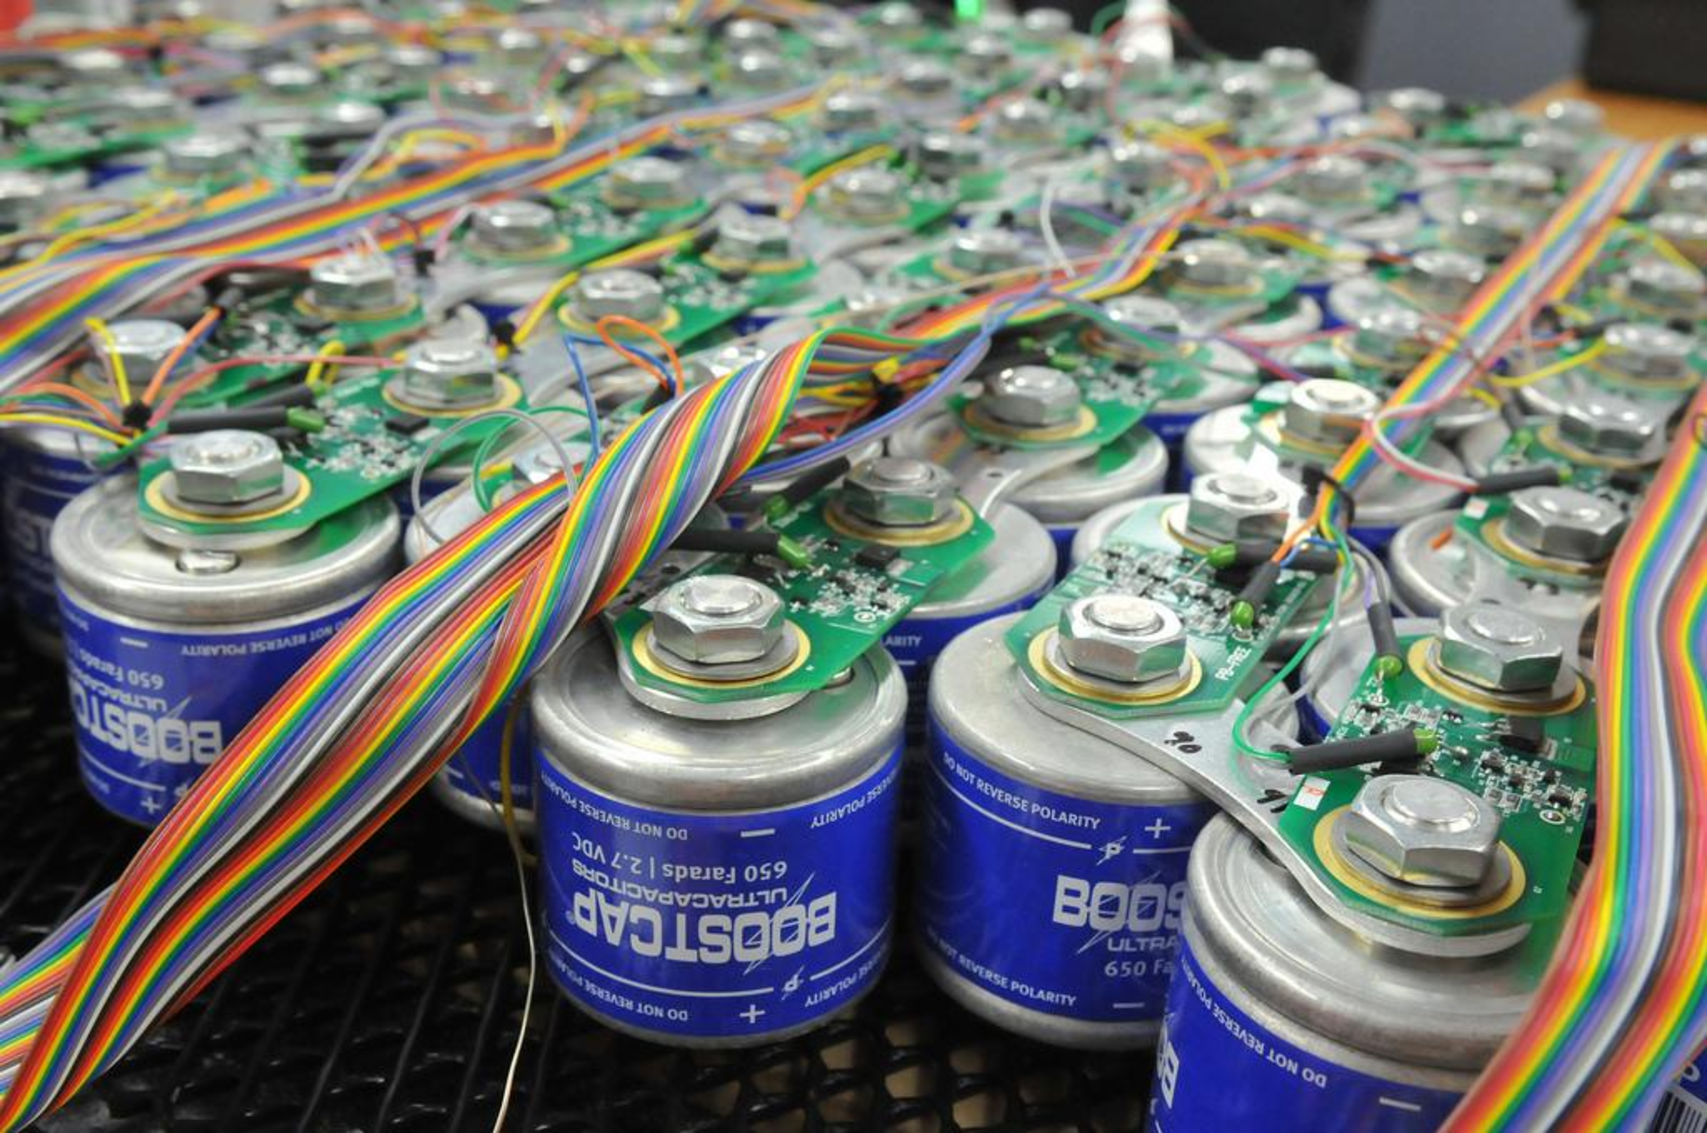
\includegraphics[width=0.9\linewidth]{ultracapacitor_banck}
\caption{Banco Ultracapacitivo com os Equalizadores de Tensão \cite{banco_ultracapacitivo}}
\label{fig:topologia_dos_equlizadores_utilizados_no_presente_trabalho}
\end{figure}

\newpage

Os componentes escolhidos para a confecção do equalizador de tensão do presente projeto é relativo ao projeto da maxwel buscando utilizar os conceitos mais
avançados de PCB, assim como componentes SMD e roteamento dupla face.\\
O componente real a ser construido é composto dos seguintes componentes : Amplificador operacional TS952IPT, amplificador operacional npn e pnp BC857B e BC847B.\\
Abaixo encontra-se a simulação do componente enquanto sua aplicação na equalização de tensão.
\begin{figure}[h!]
\centering
\includegraphics[width=0.9\linewidth]{simulacao_dipositivo_a_ser_construido}
\caption{Simulação da Versão Modelada do Equalizador de tensão em questão \textit{Fonte : Autor}}
\label{fig:topologia_dos_equlizadores_utilizados_no_presente_trabalho}
\end{figure}

O projeto PCB do componente além de sua renderização encontram-se abaixo nas figuras (\ref{Projeto_pcb_do_equalizador_proposto}) e (\ref{fig:renderizacao_do_equalizador_proposto}).

\begin{figure}[h!]
\centering
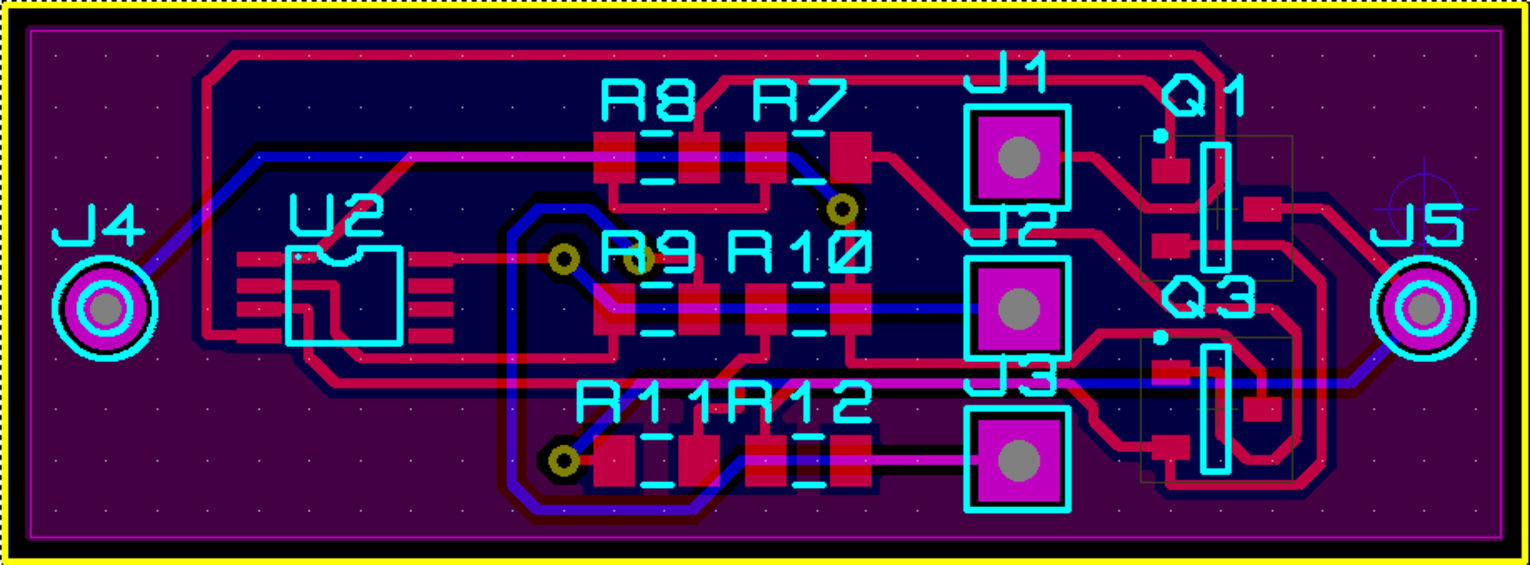
\includegraphics[width=1\linewidth]{equalizer_project}
\caption{Projeto PCB Equalizador Proposto \textit{Fonte : Autor}}
\label{Projeto_pcb_do_equalizador_proposto}
\end{figure}

\begin{figure}[h!]
\centering
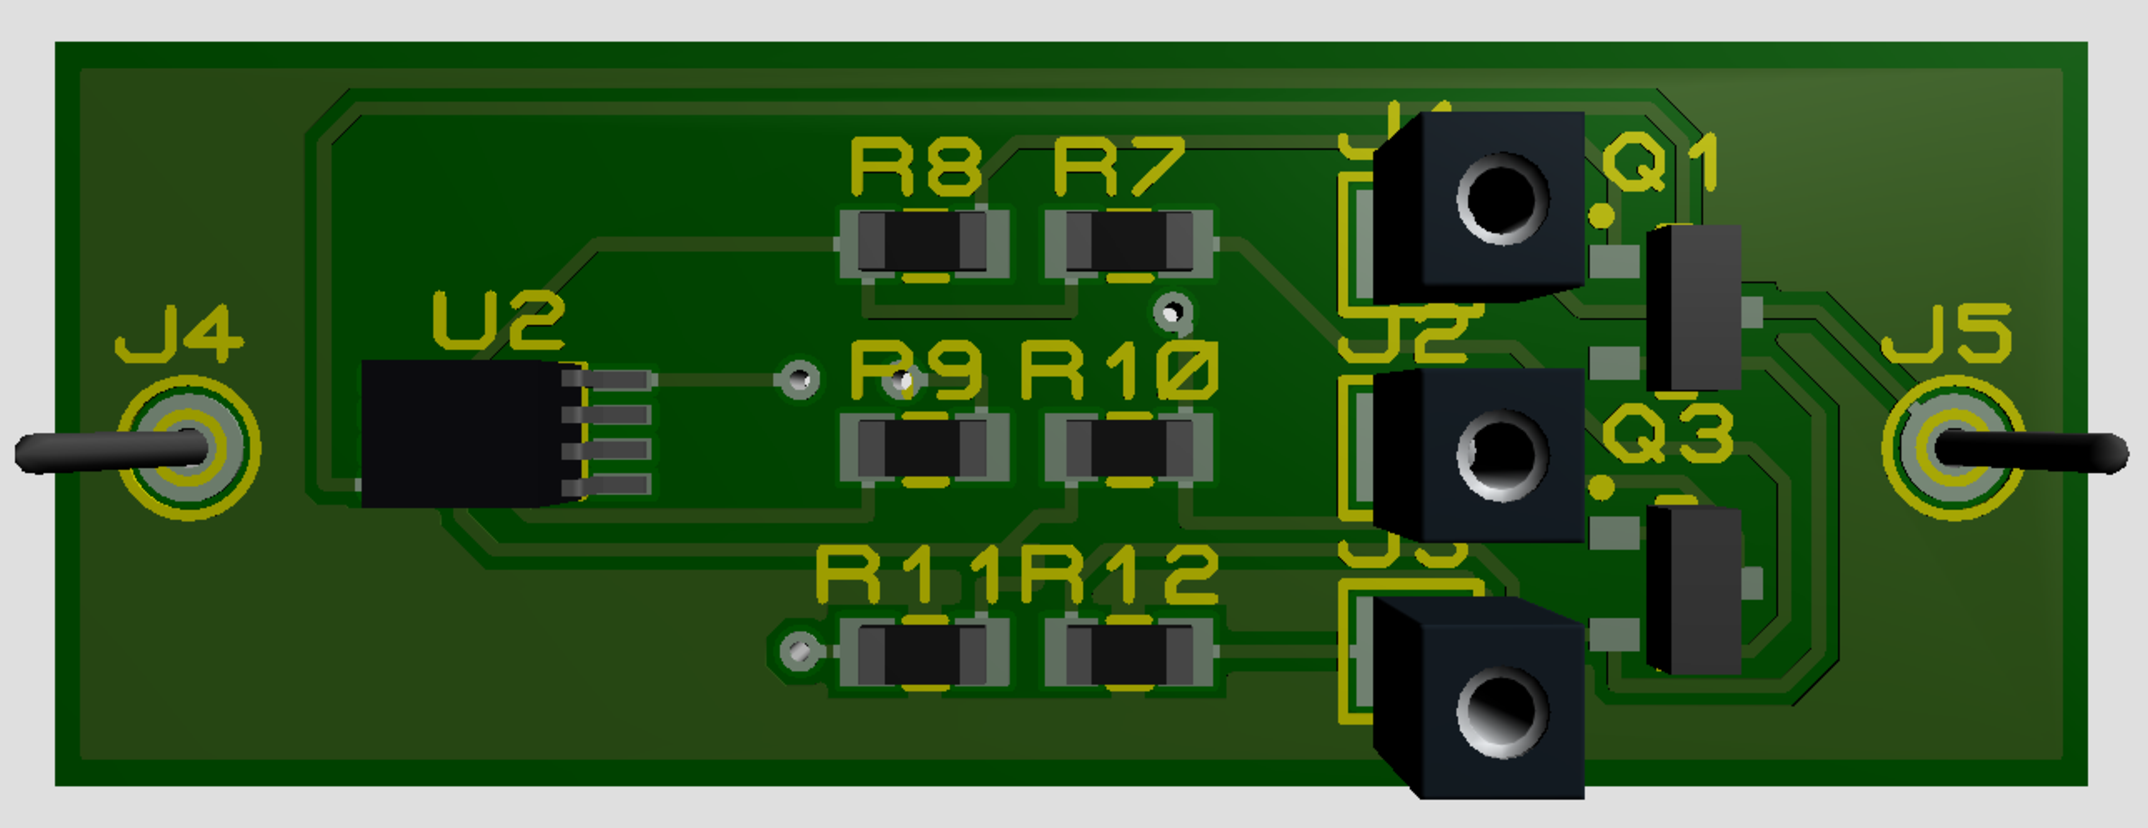
\includegraphics[width=1\linewidth]{Renderizacao_equalizer}
\caption{Renderização do Equalizador Proposto \textit{Fonte : Autor}}
\label{fig:renderizacao_do_equalizador_proposto}
\end{figure}

\section{Conclusão}
Havendo o crescimento das nações é inerente a este que a suprimissão de energia também seja concebida, afinal não vê-se futuro sem os atuais usos da elétrica.
Isto implica no profundo desenvolvimento da área tratada neste trabalho, afinal o mesmo lida com as diferentes formas de se armazenar energia em um banco 
ultracapacitivo.\\
Cabe destacar outros fatos, como o conhecimento de um ótimo laboratório e uma área em pleno crescimento. Contato com simuladores e a descrição do relatório 
se faz um desafio, de modo que houve um crescimento inerente ao mesmo que concluiu este trabalho.

\newpage

\bibliographystyle{ieeetr}
\bibliography{IC_Novo} 

\end{document} 